\documentclass[12pt]{article}
\usepackage{graphicx}
\usepackage[margin=.5in]{geometry} 
\usepackage{amsmath,amsthm,amssymb}
%\usepackage{gensymb}
  \usepackage{hyperref}
  \usepackage{pdfpages} 
  %\usepackage[table]{xcolor}
  
 %\usepackage{xcolor} % Required for specifying colors by name
\definecolor{ocre}{RGB}{52,177,201} % Define the orange color used for highlighting throughout the book

% Font Settings
\usepackage{avant} % Use the Avantgarde font for headings
%\usepackage{times} % Use the Times font for headings
\usepackage{mathptmx} % Use the Adobe Times Roman as the default text font together with math symbols from the Sym­bol, Chancery and Com­puter Modern fonts

%\usepackage{microtype} % Slightly tweak font spacing for aesthetics
%\usepackage[utf8]{inputenc} % Required for including letters with accents
\usepackage[T1]{fontenc} % Use 8-bit encoding that has 256 glyphs
%\usepackage{soul}
\usepackage{undertilde}
%\usepackage{accents}
\newcommand{\StandardLM}{\by=\bX \bbeta +{\epsilonbf}}

\usepackage{xcolor}
\usepackage{xparse}
\definecolor{lightGray}{gray}{0.95}
\definecolor{lightGrayOne}{gray}{0.9}
\definecolor{lightBlueOne}{RGB}{204, 255, 255}
\definecolor{lightBlueTwo}{RGB}{204, 238, 255}
\definecolor{lightBlueThree}{RGB}{204, 204, 255}
\definecolor{AltBlue}{RGB}{119,14,161}
\definecolor{Orchid}{RGB}{186,85,211}

\definecolor{BGBlue}{RGB}{220,221,252}
\definecolor{BGBlueOne}{RGB}{204,229,255}

\definecolor{DarkGreenOne}{RGB}{34,139,34}

\definecolor{BGGreen}{RGB}{240,243,245}
\definecolor{lightGreenOne}{RGB}{179, 255, 179}
\definecolor{lightGreenTwo}{RGB}{198, 255, 179}
\definecolor{lightGreenThree}{RGB}{243, 255, 230}
\definecolor{AltGreen}{RGB}{193, 240, 240}

\definecolor{BOGreen}{RGB}{180,0,0}
\definecolor{BGGreenOne}{RGB}{220,250,220}

\definecolor{lightBrownOne}{RGB}{255, 221, 204}
\definecolor{lightBrownTwo}{RGB}{255, 229, 204}
\definecolor{lightBrownThree}{RGB}{242, 217, 230}


\definecolor{HLTGreen}{RGB}{230,244,215}
\definecolor{ExcBrown}{RGB}{153,0,0}
\definecolor{ExcBGBrown}{RGB}{255,204,204}
\definecolor{BGYellowOne}{RGB}{255,235,208}
\definecolor{BGPink}{RGB}{255,215,240}

\newcommand{\MakeVec}[1]{{\utilde{\bf #1}}}

\NewDocumentCommand{\MCOption}{O{1.75in} m}{
\TextInBoxTwo[BGPink]{ #1 } {\TextInBoxTwo[white]{.1 in }{ \quad}\HLT{#2}}
}

 \NewDocumentCommand{\ThreeChoices}{O{Do not Know}O{Not confident}O{Confident}}{
\MCOption{#1} \MCOption{#2} \MCOption{#3}
}
 
\NewDocumentCommand{\OneBlock}{ O{HLTGreen} m m }{\colorbox{#1}{\begin{minipage}{#2} $ #3$ \end{minipage}}}

\NewDocumentCommand{\HLT}{ O{HLTGreen} m }{\colorbox{#1}{#2}}
%\NewDocumentCommand{\HLTEQ}{ O{HLTGreen} m }{\colorbox{#1}{$#2$}}
\NewDocumentCommand{\HLTEQ}{ O{white} m }{\colorbox{#1}{$#2$}}

%\newcommand{\HLT}[1]{\colorbox{HLTGreen}{#1}}
\newcommand{\DEHLT}[1]{\colorbox{lightGrayOne}{\color{white} #1}}

\newcommand{\TextInBoxOne}[2]{  {\fcolorbox{white}{lightGrayOne}{\begin{minipage}{#1}  #2 \end{minipage}}}}


\NewDocumentCommand{\TextInBoxTwo}{ O{lightGrayOne} m m } {{\fcolorbox{white}{#1}{\begin{minipage}{#2} { #3} \end{minipage}}}}


\newcommand{\TextInBox}[2]{  {\fcolorbox{BGGreen}{BGGreen}{\begin{minipage}{#1}  #2 \end{minipage}}}}
\newcommand{\TextInBoxCol}[2]{
\fcolorbox{BGBlue}{BGBlue}{%
\begin{minipage}{#1}
 {\color{AltBlue} #2}
\end{minipage}}%
}

\NewDocumentCommand{\TxtBnd}{ O{lightBrownOne} m m } {{\fcolorbox{white}{#1}{\begin{minipage}{#2} { #3} \end{minipage}}}}


\newcommand{\BandInTopBox}[2]{
\fcolorbox{AltBlue}{AltBlue}{%
\begin{minipage}{#1}{ {\color{white}  #2 \hspace{.1in}} }
\end{minipage}}%
}


\newcommand{\TextInBoxThm}[2]{
\fcolorbox{AltBlue}{lightGray}{%
\begin{minipage}{#1}
 {\color{black} #2}
\end{minipage}}%
}

\newcommand{\TextInBoxThmOne}[2]{
\fcolorbox{BGBlue}{BGBlueOne}{%
\begin{minipage}{#1}
 {\color{AltBlue} #2}
\end{minipage}}%
}

\newcommand{\TextInBoxLem}[2]{
\fcolorbox{BGBlue}{lightGray}{%
\begin{minipage}{#1}
 {\color{black} #2}
\end{minipage}}%
}



\newcommand{\TextInBoxLemOne}[2]{
\vspace{.02 in}
\noindent
\fcolorbox{BGBlue}{BGBlue}{%
\begin{minipage}{#1}
 {\color{AltBlue} #2}
\end{minipage}}%
}



\newcommand{\DefBox}[1]{
%\vspace{.1 in}
\noindent
\TextInBoxLem{4.5 in }{
\BandInTopBox{4.4 in }{}
\TextInBoxLemOne{4.4 in }{
#1
}}}





\newcommand{\DefBoxOne}[2]{
%\vspace{.1 in}
\noindent
\TextInBoxLem{4.5 in }{
\BandInTopBox{4.4 in }{#1}
\TextInBoxLemOne{4.4 in }{
#2
}}}


\newcommand{\ThmBox}[2]{
\noindent
\TextInBoxThm{4.4 in }{
\TextInBoxThmOne{4.4 in }{
#1}
#2}
}

\newcommand{\LemBox}[2]{
\noindent
\TextInBoxLem{4.5 in }{
\TextInBoxLemOne{4.4 in }{
#1}
#2}
}

\newcommand{\PropBox}[2]{
\vspace{.1 in}
\noindent
\TextInBoxLem{4.5 in }{
\TextInBoxLemOne{4.4 in }{
#1}
#2}
}




\newcommand{\TextInBoxExc}[2]{
\noindent
\fcolorbox{white}{BGGreenOne}{%
\begin{minipage}{#1}
 {\color{black} #2}
\end{minipage}}%
}


\newcommand{\TextInBoxExample}[2]{
\noindent
\fcolorbox{white}{BGPink}{%
\begin{minipage}{#1}
 {\color{black} #2}
\end{minipage}}%
}


\newcommand{\ExerciseBox}[1]{
\noindent
%\TextInBoxLem{6 in }{
\TextInBoxExc{6 in }{
#1}
%#2}
}


\newcommand{\ExampleBox}[1]{
\noindent
%\TextInBoxLem{6 in }{
\TextInBoxExample{6 in }{
#1}
%#2}
}

\NewDocumentCommand{\CommentBox}{ O{BGBlue}  m }{
\TextInBoxLem{5.5in }{
{\bf Comment:}\\
\TextInBoxLemOne{5.4 in }{
#2}}
}



\newcommand{\HLTY}[1]{\HLTEQ[yellow]{#1}}
\newcommand{\HLTW}[1]{\HLTEQ[white]{#1}}



\newcommand{\qBox}[1]{
  \begin{tikzpicture}
\node[draw=none,shade,
      top color=lightGrayOne,
      bottom color=lightGray,
      rounded corners=2pt,
      blur shadow={shadow blur steps=5}
    ] at (0,0) {    \noindent 
\fcolorbox{white}{BGBlue}{%
\begin{minipage}{4.55 in}
 {\color{black} {
 #1}}
\end{minipage}  }%
 };
 
    \end{tikzpicture}
}
 
 


 

\newcommand{\qBoxCol}[2]{
  \begin{tikzpicture}
\node[draw=none,shade,
      top color=lightGrayOne,
      bottom color=lightGray,
      rounded corners=2pt,
      blur shadow={shadow blur steps=5}
    ] at (0,0) {    \noindent
\fcolorbox{white}{#1}{%
%\begin{minipage}{4.55 in}
\begin{minipage}{4.55 in}
 {
 \color{black} {
 #2}}
\end{minipage}  }%
 };
 
    \end{tikzpicture}
}
  
  
  
  
  
  

\NewDocumentCommand{\qBrd}{O{4.55 in} m m}{
  \begin{tikzpicture}
\node[draw=none,shade,
      top color=#2,
      bottom color=#2,
      rounded corners=2pt,
      blur shadow={shadow blur steps=5}
    ] at (0,0) {    \begin{minipage}{#1}
 {
 \color{black} {
 #3}}
\end{minipage} 

 };
 
    \end{tikzpicture}
}
    
  
  
  
  
\NewDocumentCommand{\qbx}{O{4.55 in} m m}{
  \begin{tikzpicture}
\node[draw=none,shade,
      top color=lightGrayOne,
      bottom color=lightGray,
      rounded corners=2pt,
      blur shadow={shadow blur steps=5}
    ] at (0,0) {    \noindent
\fcolorbox{white}{#2}{%
%\begin{minipage}{4.55 in}
\begin{minipage}{#1}
 {
 \color{black} {
 #3}}
\end{minipage}  }%
 };
 
    \end{tikzpicture}
}
  
 
 
 \newcommand{\CurlyBox}[1]{
\begin{center}
  \begin{tikzpicture}
    \node[tape,draw=none,shade,
      top color=blue!40,
      bottom color=blue!5,
      rounded corners=1pt,
      blur shadow={shadow blur steps=5,shadow blur extra rounding=1.3pt}
    ] at (2,0){\sffamily\bfseries\large #1};
  \end{tikzpicture}
\end{center} 
 }


\newcommand{\CmntBnd}{\BandInTopBox{4.5in}{Comment:}}
\NewDocumentCommand{\TopBand}{O{Comment:} m}{ \BandInTopBox{4.5in}{#2}}

\newcommand{\DBX}[1]{
 	\HLTEQ[AltBlue]{
 				\HLTEQ[BGBlue]{  #1  }
 	}
 }



\NewDocumentCommand{\TransitionFrame}{O{slateblue}m}{
\begin{frame}{ }
\qBoxCol{#1!40}{\vspace{.8in}  \begin{center}\qBrd[2in]{#1!70}{ \begin{center} \vspace{.1in}
  #2 \\
 \vspace{.1in}
\end{center}}\end{center}
\vspace{.7in}
}

\end{frame}

}
%\newcommand{\proof}{ {\bf Proof:  } }
%\usepackage{enumerate}
%
\NewDocumentCommand{\InnerProduct}{ O{\cdot,\cdot} }{ \left\langle #1  \right\rangle  }

%\newcommand{\InnerProduct}[2]{  \left\langle #1, #2  \right\rangle }
\newcommand{\Ind}[1]{\mathbb{I}\left(#1 \right)}
\newcommand{\StandardLM}{\by=\bX \bbeta +{\epsilonbf}}
\newcommand{\StandardLMmod}{\bY=\bX \bbeta +{\epsilonbf}}
\usepackage{undertilde}
\newcommand{\MakeVec}[1]{{\utilde{\bf #1}}}
\newcommand{\Zplus}{{\Z_{+}}}
\newcommand{\Proj}[1]{{#1}\left( {#1}^T{#1}\right)^{-}{#1}^T }
\NewDocumentCommand{\YiDotDef}{O{B} m}{ \left(Y_{{#2}1},\ldots,Y_{{#2}{#1}} \right)}
\NewDocumentCommand{\YiDot}{O{i}}{  \utilde{Y}_{{#1 \bullet}}  }

\NewDocumentCommand{\OneWay}{ O{T} O{B} m}{
 \IfEqCase{#3}{%
  {model}{   Y_{ij}=\mu+ \tau_i+ \epsilon_{ij} \text{ for } i 		=1, 2,\ldots #1; j = 1,2,\ldots #2  
  	 }
  {Y}{
  \left[ {\begin{array}{c;{2pt/2pt}c;{2pt/2pt}c;{2pt/2pt}c ;{2pt/2pt}c}
   \overbrace{ Y_{11},\ldots ,Y_{1{#2}}}^{\text{Treatment 1}}  & \cdots &  \overbrace{ Y_{i1},\ldots Y_{i{#2}}}^{\text{Treatment 2}} & \cdots & \overbrace{Y_{{#1}1} \ldots Y_{{{#1}}{#2}}}^{\text{Treatment #1}} \end{array} } \right]^T 
  	 }
  	 {YInDot}{\left[ {\begin{array}{c;{2pt/2pt}c;{2pt/2pt}c;{2pt/2pt}c ;{2pt/2pt}c}
  \utilde{Y}_{1 \bullet}^T  & \cdots &   \utilde{Y}_{i \bullet}^T& \cdots & \utilde{Y}_{{#1} \bullet}^T \end{array} } \right]^T_{{#1}{#2}\times 1}
  	 }
  	 {response}{
  \left[ {\begin{array}{c;{2pt/2pt}c;{2pt/2pt}c;{2pt/2pt}c ;{2pt/2pt}c}
   \overbrace{ Y_{11},\ldots ,Y_{1{#2}}}^{\text{Treatment 1}}  & \cdots &  \overbrace{ Y_{i1},\ldots Y_{i{#2}}}^{\text{Treatment 2}} & \cdots & \overbrace{Y_{{#1}1} \ldots Y_{{{#1}}{#2}}}^{\text{Treatment #1}} \end{array} } \right]^T  
  	 }
  	 {treatments}{ \tau_1,\ldots , \tau_{#1} }
  	  {tau}{ \tau_1,\ldots , \tau_{#1} }
  	 {beta}{\left(\mu, \HLT{$\tau_1,\ldots , \tau_{#1} $}\right)^T}
  	 {error}{
  \left[ {\begin{array}{c;{2pt/2pt}c;{2pt/2pt}c;{2pt/2pt}c ;{2pt/2pt}c}
   \overbrace{ \epsilon_{11},\ldots ,\epsilon_{1{#2}}}^{\text{Treatment 1}}  & \cdots &  \overbrace{ \epsilon_{i1},\ldots \epsilon_{i{#2}}}^{\text{Treatment 2}} & \cdots & \overbrace{\epsilon_{{#1}1} \ldots \epsilon_{{{#1}}{#2}}}^{\text{Treatment #1}} \end{array} } \right]^T   
  	 }
  	 {design}{
 \left[ {\begin{array}{c;{2pt/2pt}cccc}
   \Onebf_{#2} &  \Onebf_{#2} & \ZeroF  & \ldots &  \ZeroF\\
   \Onebf_{#2} &  \ZeroF   &\Onebf_{#2} & \ldots  & \ZeroF\\
   \vdots   & \vdots    & \vdots  & \ddots & \vdots  \\
    \Onebf_{#2} & \ZeroF & \cdots  & \ldots    & \Onebf_{#2}\\
    \end{array}
   } \right] _{{#1}{#2}\times ({#1}+1)}
  }
  {designKP}{ \left[  {\begin{array}{c;{2pt/2pt}c}
   \underbrace{\Onebf_{#1}\otimes  \Onebf_{#2}} &  \underbrace{I_{#1} \otimes \Onebf_{#2} }
   \end{array} }\right]
   }
    {X}{
 \left[ {\begin{array}{c;{2pt/2pt}cccc}
   \Onebf_{#2} &  \Onebf_{#2} & \ZeroF  & \ldots &  \ZeroF\\
   \Onebf_{#2} &  \ZeroF   &\Onebf_{#2} & \ldots  & \ZeroF\\
   \vdots   & \vdots    & \vdots  & \ddots & \vdots  \\
    \Onebf_{#2} & \ZeroF & \cdots  & \ldots    & \Onebf_{#2}\\
    \end{array}
   } \right] _{{#1}{#2}\times ({#1}+1)}
  }
  {XKP}{ \left[  {\begin{array}{c;{2pt/2pt}c}
   \underbrace{\Onebf_{#1}\otimes  \Onebf_{#2}} &  \underbrace{I_{{#1}} \otimes \Onebf_{#2} }
   \end{array} }\right]
   }
   {XMu}{ \Onebf_{#1}\otimes  \Onebf_{#2} }
   {XTau}{I_{{#1}} \otimes \Onebf_{#2}}
   {ProjMat}{
   \left[ {\begin{array}{c;{2pt/2pt}c;{2pt/2pt}c ;{2pt/2pt}c}
    \HLT{$\ProjOne{#2}$}&  \ZeroF& \cdots &\ZeroF\\
   \ZeroF&  \HLT{$\ProjOne{#2}$} & \cdots & \ZeroF\\
   \vdots &\vdots  &  \vdots   & \vdots  \\
    \ZeroF&  \ZeroF & \cdots & \HLT{$\ProjOne{#2}$}
    \end{array}
   } \right]_{{#1}{#2}\times {#1}{#2} }
   }
    {ProjMatKP}{
    I_{#1}\otimes {\ProjOne{#2}}
    }
    {YColVec}{
    \left[ {\begin{array}{c}
  \utilde{Y}_{1 \bullet}\\
  \hdashline[2pt/2pt]\\
   \vdots\\
  \hdashline[2pt/2pt]\\
  \utilde{Y}_{i \bullet}\\
  \hdashline[2pt/2pt]\\
   \vdots\\
  \hdashline[2pt/2pt]\\
   \utilde{Y}_{{#1} \bullet}\\
    \end{array}
   } \right]_{{#1}{#2}\times 1}}
   {YDotBar}{\left[
   {\begin{array}{c}
  \overline{Y}_{1 \bullet}\\
  \hdashline[2pt/2pt]\\
   \vdots\\
  \hdashline[2pt/2pt]\\
  \overline{Y}_{i \bullet}\\
  \hdashline[2pt/2pt]\\
   \vdots\\
  \hdashline[2pt/2pt]\\
   \overline{Y}_{{#1} \bullet}\\
    \end{array}
   }\right]_{{#1}\times 1} }
    }  	 
}







%
%
%%\usepackage{accents}
%\newcommand{\SpaceU}{\mathcal{U}}
%\newcommand{\Span}[1]{\mathcal{L}(#1)}
%%\hypersetup{colorlinks=true}
%\newcommand{\N}{\mathbb{N}}
%\newcommand{\Z}{\mathbb{Z}}
% \newcommand{\SpaceW}{\mathcal{W}}
%\newcommand{\SpaceV}{\mathcal{V}}
%\newcommand{\real}[1]{{\mathbb R}^{#1}}
%\newcommand{\Pdg}{P_{\alphabfs (\Deltabfs_{y})}}
%\newcommand{\spn}{\mathrm{span}}
%\newcommand{\diag}{\mathrm{diag}}
\newcommand{\E}{\mathrm{E}}
\newcommand{\var}{\mathrm{Var}}
\newcommand{\cov}{\mathrm{Cov}}
\newcommand{\covhat}{\widehat{\mathrm{Cov}}}
\newcommand{\rank}{\mathrm{rank}}
\newcommand{\stack}{\mathrm{stack}}
\newcommand{\Normal}{\mathrm{Normal}}
\newcommand{\tr}{\mathrm{\,tr}}
\newcommand{\avar}{\mathrm{\,avar}}
\newcommand{\vecc}{\mathrm{\,vec}}
\newcommand{\true}{\mathrm{true}}

% Bold Face symbols
\newcommand{\vbf}{{\mathbf v}}
\newcommand{\w}{{\utilde{\mathbf w}}}
\newcommand{\X}{\mathbf X}
\newcommand{\Xhat}{\widehat{\X}}
\newcommand{\x}{{\utilde{\mathbf x}}}
\newcommand{\Y}{{\mathbf Y}}
\newcommand{\y}{\mathbf y}
\newcommand{\Xbar}{\bar{\X}}
\newcommand{\Ybar}{\bar{\Y}}
\newcommand{\ellhat}{\hat{\ell}}
\newcommand{\ellbf}{\mathbf{\ell}}
\newcommand{\ellbfhat}{\hat{\ellbf}}
\newcommand{\abf}{{\utilde{\mathbf a}}}
\newcommand{\q}{{\mathbf q}}
\newcommand{\f}{{\mathbf f}}
\newcommand{\Obf}{\mathbf O}


\newcommand{\Xcaln}{{\mathcal X}_{n}}
\newcommand{\Xbarcal}{\bar{{\mathcal X}}}
\newcommand{\Xbb}{\mathbb{X}}
\newcommand{\Fbb}{\mathbb{F}}
\newcommand{\Ybb}{\mathbb{Y}}

\newcommand{\Xbbhat}{\widehat{\mathbb{X}}}
\newcommand{\Ss}{\mathbf{S}}
\newcommand{\Ty}{\T_{y}}
\makeatletter
\renewcommand*{\@seccntformat}[1]{%
   \csname the#1\endcsname.\quad}
\makeatother
%\newcommand{\Z}{{\mathbf Z}}
\newcommand{\z}{{\mathbf z}}
\newcommand{\Zbar}{\bar{\Z}}
\newcommand{\Zhat}{\hat{\Z}}
\newcommand{\Zwidehat}{\widehat{\Z}}
\newcommand{\Sigmabfhatz}{\greekbold{\hat{\Sigma}}_{\Z}}
\newcommand{\Sigmabfhatzy}{\greekbold{\hat{\Sigma}}_{\Z|y}}
\newcommand{\Sigmabfzy}{\Sigmabf_{\Z|y}}
\newcommand{\sigmahat}{\hat{\sigma}}

\newcommand{\fit}{\mathrm{fit}}
\newcommand{\res}{\mathrm{res}}
\newcommand{\rres}{{ 11},\mathrm{res}}

\newcommand{\ffit}{{ 11},\mathrm{fit}}
\newcommand{\G}{\mathbf{G}}
\newcommand{\Ll}{\mathbf{L}}
\newcommand{\Guno}{\mathbf{G_1}}
\newcommand{\Hh}{\mathbf{H}}
\newcommand{\Ww}{\mathbf{W}}
\newcommand{\Mm}{\mathbf{M}}
\newcommand{\bw}{{\utilde{\mathbf{w}}}}


%\newcommand{\pfcpc}{PFC(PC)}
\newcommand{\pfcpc}{$\mathrm{PFC}_{\mathrm{PC}}$}
\newcommand{\pfcall}{$\mathrm{PFC}_{\mathrm{all}}$}

\newcommand{\fbf}{{\mathbf f}}
\newcommand{\fbfhat}{\hat{\fbf}}
\newcommand{\fhat}{\hat{f}}
\newcommand{\D}{\mathbf D}
\newcommand{\cbf}{{\mathbf c}}
\newcommand{\Dfbf}{\D_{\fbf}}
\newcommand{\Dfbfhat}{\D_{\fbfhat}}
\newcommand{\K}{\mathbf K}
\newcommand{\Khat}{\widehat \K}

\newcommand{\ghat}{\hat{g}}
\newcommand{\Bhat}{\widehat{\B}}
\newcommand{\Rhat}{\widehat{R}}
\newcommand{\vhat}{\widehat{\bv}}

\newcommand{\uhat}{\widehat{\bu}}
\newcommand{\gbf}{{\mathbf g}}
\newcommand{\gbfhat}{\hat{\gbf}}

\newcommand{\Dgbf}{\D_{\gbf}}
\newcommand{\Dgbfhat}{\D_{\gbfhat}}

\newcommand{\obf}{\mathbf o}
\newcommand{\Pbf}{{\mathbf P}}
\newcommand{\Qbf}{{\mathbf Q}}
\newcommand{\Qfbf}{\Qbf_{\fbf}}
\newcommand{\Qfbfhat}{\Qbf_{\fbfhat}}
\newcommand{\Qgbf}{\Qbf_{\gbf}}
\newcommand{\Qgbfhat}{\Qbf_{\gbfhat}}
\newcommand{\Pgbf}{\Pbf_{\gbf}}

\newcommand{\T}{\mathbf T}
\newcommand{\tT}{\widetilde{\T}}
\newcommand{\tV}{\widetilde{\V}}
\newcommand{\dT}{\dot{\T}}
\newcommand{\dV}{\dot{\V}}
\newcommand{\ddT}{\ddot{\T}}
\newcommand{\V}{{\mathbf V}}
\newcommand{\Vhat}{\widehat \V}
%\newcommand{\bv}{{\utilde{\mathbf v}}}
\newcommand{\bu}{{\utilde{\mathbf u}}}
\newcommand{\Vhalf}{{\mathbf V}^{\half}}
\newcommand{\tL}{{\widetilde L}}
%\newcommand{\bd}{\deltabf}

\newcommand{\ahat}{{\hat{a}}}
\newcommand{\bhat}{{\hat{b}}}

\newcommand{\U}{{\mathbf U}}
\newcommand{\tD}{{\tilde{D}}}
\newcommand{\W}{{\mathbf W}}
\newcommand{\dbf}{{\mathbf d}}
\newcommand{\Lbf}{{\mathbf L}}
\newcommand{\F}{{\mathbf F}}
\newcommand{\M}{{\mathbf M}}
%\newcommand{\N}{{\mathbf N}}
\newcommand{\s}{{\mathbf S}}
\newcommand{\sy}{{\mathbf S}_{y}}
\newcommand{\bbf}{{\utilde{\mathbf b}}}
\newcommand{\A}{{\mathbf A}}
\newcommand{\B}{{\mathbf B}}
\newcommand{\Q}{{\mathbf Q}}
\newcommand{\C}{{\mathbf C}}
\newcommand{\Chat}{\widehat{\mathbf C}}
\newcommand{\Dhat}{\widehat{\mathbf D}}
\newcommand{\e}{\utilde{\mathbf e}}
\newcommand{\Ebf}{{\mathbf E}}
\newcommand{\g}{\mathbf g}
\newcommand{\R}{{\mathbb{ R}}}
\newcommand{\Ghat}{\widehat{\G}}
\newcommand{\Hbf}{{\mathbf H}}
\newcommand{\h}{\mathbf h}
\newcommand{\tB}{\widetilde{\B}}
\newcommand{\tC}{\widetilde{\C}}
\newcommand{\mpc}{M_{\mathrm{\scriptscriptstyle{PC}}}}
\newcommand{\mpfc}{M_{\mathrm{\scriptscriptstyle{PFC}}}}
\newcommand{\lpc}{L_{\mathrm{\scriptscriptstyle{PC}}}}
\newcommand{\lpfc}{L_{\mathrm{\scriptscriptstyle{PFC}}}}
\newcommand{\tlpfc}{\widetilde{L}_{\mathrm{\scriptscriptstyle{PFC}}}}



% Greek Bold Face symbols

\newcommand{\greekbold}[1]{\mbox{\boldmath $#1$}}
\newcommand{\alphabf}{{\utilde{\greekbold{\alpha}}}}
\newcommand{\alphabfhat}{\widehat{\alphabf}}
\newcommand{\alphahat}{\widehat{\alpha}}
\newcommand{\alphabfs}{\greekbold{\scriptstyle \alpha}}
\newcommand{\etabf}{\utilde{\greekbold{\eta}}}
\newcommand{\etabftd}{\widetilde{\etabf}}
\newcommand{\etabfs}{\greekbold{\scriptstyle \eta}}
\newcommand{\betabf}{\utilde{\greekbold{\beta}}}
%\newcommand{\taubf}{\utilde{\greekbold{\tau}}}
\newcommand{\lambdabf}{\utilde{\greekbold{\lambda}}}
\newcommand{\etabfhat}{\hat{\greekbold{\eta}}}
\newcommand{\rhobf}{\greekbold{\rho}}
\newcommand{\betabfhat}{\widehat{\greekbold{\beta}}}
\newcommand{\betabfs}{\greekbold{\scriptstyle \beta}}
\newcommand{\taubfhat}{\hat{\greekbold{\tau}}}
\newcommand{\taubfn}{\taubf_{n}}
\newcommand{\taubfhatn}{\hat{\taubf}_{n}}
\newcommand{\Lambdabf}{\greekbold{\Lambda}}
\newcommand{\Lambdabfhat}{\widehat{\greekbold{\Lambda}}}
\newcommand{\Lambdabfs}{\greekbold{\scriptstyle{\Lambda}}}
\newcommand{\epsilonbf}{{\utilde{\greekbold{\epsilon}}}}
\newcommand{\mubfbar}{\bar{\mubf}}
\newcommand{\mubfhat}{\hat{\mubf}}
\newcommand{\mubfs}{{\greekbold{\scriptstyle \mu}}}
\newcommand{\J}{\mathbf J}
\newcommand{\gammabf}{\greekbold{\gamma}}
\newcommand{\gammabfhat}{\hat{\greekbold{\gamma}}}
\newcommand{\gammabfy}{\greekbold{\gamma}_{y}}
\newcommand{\Gammabf}{\greekbold{\Gamma}}
\newcommand{\Gammabft}{\widetilde{\greekbold{\Gamma}}}
\newcommand{\gammabfs}{\greekbold{{\scriptstyle \gamma}}}
\newcommand{\Gammabfs}{{\greekbold{\scriptstyle \Gamma}}}
\newcommand{\Gammabfhat}{\widehat{\greekbold{\Gamma}}}
\newcommand{\deltabf}{\greekbold{\delta}}
\newcommand{\Deltabf}{\greekbold{\Delta}}
\newcommand{\Deltabfhat}{\widehat{\greekbold{\Delta}}}
\newcommand{\Deltabfs}{{\greekbold{\scriptstyle \Delta}}}
\newcommand{\deltabfs}{{\greekbold{\scriptstyle \delta}}}
\newcommand{\Deltabfshat}{{\widehat{\greekbold{\scriptstyle \Delta}}}}
\newcommand{\omegabf}{\greekbold{\omega}}
\newcommand{\Omegabf}{\greekbold{\Omega}}
\newcommand{\Omegabft}{\widetilde{\greekbold{\Omega}}}
\newcommand{\Omegabfs}{{\greekbold{\scriptstyle \Omega}}}
\newcommand{\Omegabfstd}{{\tilde{\greekbold{\scriptstyle \Omegabf}}}}
\newcommand{\Omegabfsbar}{{\bar{\greekbold{\scriptstyle{\Omegabf}}}}}
\newcommand{\Omegabftd}{\widetilde{\Omegabf}}
\newcommand{\Omegabfbar}{\bar{\Omegabf}}
\newcommand{\Omegabfhat}{\widehat{\greekbold{\Omega}}}
\newcommand{\phibf}{\greekbold{\phi}}
\newcommand{\phibfhat}{\hat{\greekbold{\phi}}}


\newcommand{\Sigmabf}{\greekbold{\Sigma}}
\newcommand{\Sigmabfhat}{\greekbold{\widehat{\Sigma}}}
\newcommand{\Sigmabft}{\greekbold{\widetilde{\Sigma}}}
\newcommand{\Sigmabfhats}{{\greekbold{\scriptstyle \widehat{\Sigma}}}}
\newcommand{\Sigmabfs}{{\greekbold{\scriptstyle \Sigma}}}
\newcommand{\mubf}{\utilde{\greekbold{\mu}}}

\newcommand{\xibf}{\greekbold{\xi}}
\newcommand{\xibfy}{\xibf_{y}}
\newcommand{\xibfs}{{\greekbold{\scriptstyle \xi}}}
\newcommand{\xibfhat}{{\hat{\xibf}}}
\newcommand{\xibfhats}{\hat{\xibfs}}

\newcommand{\xibfhaty}{{\hat{\xibf}_{y}}}
\newcommand{\txibf}{\tilde{\greekbold{\xi}}}
\newcommand{\txibfs}{\tilde{\greekbold{\scriptstyle \xi}}}
\newcommand{\Phibf}{\greekbold{\Phi}}
\newcommand{\Phibfhat}{\widehat{\Phibf}}
\newcommand{\Phibfs}{\greekbold{\scriptstyle \Phi}}
\newcommand{\Phibfshat}{\hat{\Phibfs}}
%\newcommand{\thetabf}{\utilde{\greekbold{\theta}}}
\newcommand{\varepsilonbf}{\greekbold{\varepsilon}}

\newcommand{\zetabf}{\greekbold{\zeta}}
\newcommand{\tzetabf}{\tilde{\greekbold{\zeta}}}
\newcommand{\zetabfhat}{{\hat{\zetabf}}}
\newcommand{\zetabfs}{{\greekbold{\scriptstyle \zeta}}}
\newcommand{\zetabfhats}{\hat{\zetabfs}}
\newcommand{\nubf}{\greekbold{\nu}}
\newcommand{\nubfhat}{{\hat{\nubf}}}

\newcommand{\lambdahat}{\hat{\lambda}}
\newcommand{\ic}{(i)}

\newcommand{\fa}[1]{2{#1}}
\newcommand{\fb}[1]{1{#1}}
\newcommand{\Si}[1]{\Gammabf_{#1}\Omegabf_{#1}\Gammabf_{#1}^{T}}
\newcommand{\Sinv}[1]{\Gammabf_{#1}\Omegabf_{#1}^{-1}\Gammabf_{#1}^{T}}


%subspace notation
\newcommand{\syx}{\mathcal{S}_{Y|\X}}
\newcommand{\syz}{\mathcal{S}_{Y|\Z}}
\newcommand{\spc}{{\mathcal S}}
\newcommand{\spchat}{\widehat{\mathcal S}}
\newcommand{\dist}{{\mathcal D}}
\newcommand{\Mhat}{\widehat{{\mathbf M}}}
\newcommand{\Mhatsir}{\widehat{\mathbf M}_{\mathrm{\scriptscriptstyle{SIR}}}}
\newcommand{\Msir}{\mathbf{M}_{\mathrm{\scriptscriptstyle{SIR}}}}
\newcommand{\Msave}{\mathbf{M}_{\mathrm{\scriptscriptstyle{SAVE}}}}
\newcommand{\Mhatsave}{\widehat{\mathbf M}_{\mathrm{\scriptscriptstyle{SAVE}}}}
\newcommand{\ospc}{{\mathcal O}}
\newcommand{\hspc}{{\mathcal H}}
\newcommand{\gspc}{{\mathcal G}}
\newcommand{\mspc}{{\mathcal M}}
\newcommand{\ols}{\mathrm{ols}}
\newcommand{\pfc}{\mathrm{pfc}}
\newcommand{\mse}{\mathrm{MSE}}
\newcommand{\bspc}{\mathcal B}
\newcommand{\espc}{{\cal E}}
\newcommand{\vspc}{{\mathcal V}}
\newcommand{\iseb}{{\cal IE}_{\Sigmabfs}(\bspc)}
\newcommand{\seb}{{\cal E}_{\Sigmabfs}(\bspc)}
\newcommand{\sebhat}{\widehat{{\cal E}}_{\Sigmabfs}(\bspc)}
\newcommand{\sebp}{{\cal E}_{\Sigmabfs}(\bspc_{1})}
\newcommand{\indep}{\;\, \rule[0em]{.03em}{.67em} \hspace{-.25em}
\rule[0em]{.65em}{.03em} \hspace{-.25em}
\rule[0em]{.03em}{.67em}\;\,}
\newcommand{\iespc}{{\cal IE}}
\newcommand{\isebp}{{\cal IE}_{\Sigmabfs}^{\perp}(\bspc)}
\newcommand{\isebjhat}[1]{\widehat{{\cal IE}}_{\Sigmabfs}(\bspc)}
%\newcommand{\ZeroF}{{\bf 0}}
\newcommand{\Onebf}{{\utilde{\bf 1}}}
%\newcommand{\Onebf}{ {\underaccent{\sim}{\bf 1}}}
%\newcommand{\Ll}{\underaccent{\sim}{ l}}
%\newcommand{\ZeroF}{ {\underaccent{\sim}{\bf 0}}}
\newcommand{\ZeroF}{{\utilde{\bf 0}}}
\newcommand{\ProjOne}[1]{\frac{\Onebf_{#1} \Onebf_{#1}^T}{#1} }
\newcommand{\ProjOneK}{\frac{\Onebf_K \Onebf_K^T}{K} }

%\newtheorem{prop}{Proposition}
%\newtheorem{lemma}{Lemma}
%\newtheorem{Lemma}{Lemma}
%\newtheorem{proof}{Proof}



\newcommand{\bI}{ { \bf I }}
%\newcommand{\bX}{ \utilde{ \bf X }}
%\newcommand{\bx}{ {\utilde{ \bf x }}}
%\newcommand{\bY}{ \utilde{ \bf Y }}
%\newcommand{\bt}{ \utilde{ \bf t }}
%\newcommand{\by}{ {\utilde{ \bf y} }}
%\newcommand{\bZ}{ \utilde{ \bf Z }}
%\newcommand{\bz}{ {\utilde{ \bf z }}}
\newcommand{\bzero}{ {\utilde{ \bf 0 }}}
\newcommand{\ba}{ \utilde{ \textit{\textbf{a}}}}
\newcommand{\bb}{ \utilde{ \textit{\textbf{b}}}}
\newcommand{\EE}{\text{E}}
\newcommand{\Var}{\text{Var}}
\newcommand{\bbeta}{\utilde{\boldsymbol \beta}}
\newcommand{\bOmega}{\mbox{\boldmath{$\Omega$}}}
\newcommand{\bpsi}{\mbox{\boldmath{$\psi$}}}
\newcommand{\btheta}{\utilde{\boldsymbol \theta}}
\newcommand{\sC}{ {\cal C} }
\newcommand{\sM}{ {\cal M} }
\newcommand{\sX}{ {\cal X} }
\newcommand{\sY}{ {\cal Y} }
\newcommand{\sZ}{ {\cal Z} }
\newcommand{\ee}[1]{\mathrm{e}^{ #1 }}
\newcommand{\pr}{\text{pr}}
\newcommand{\RE}{\mathbb{R}}
\newcommand{\bigqm}[1][1]{\text{\larger[#1]{\textbf{?}}}}

\newcommand{\vsa}{\vspace{.05 in}}
\newcommand{\vsb}{\vspace{2 em}}
\newcommand{\vsc}{\vspace{1 em}}
\usepackage{color,soul}


\newcommand*\bigcdot{\mathpalette\bigcdot@{.7}}
%\newcommand*\bigcdot@[2]{\mathbin{\vcenter{\hbox{\scalebox{#2}{$\m@th#1\bullet$}}}}}
\makeatother
 
 \newcommand{\RowVecSymbol}[2]{  \left(\begin{array}{c}\rvert\\{#1}_{#2,\bigcdot}\\\rvert\end{array}\right)  }
 \newcommand{\ColumnVecSymbol}[2]{  \left(\begin{array}{c}\rvert\\{#1}_{\bigcdot,#2}\\\rvert\end{array}\right)  }
 \newcommand{\ColumnVecSymbolNoBracket}[2]{  \begin{array}{c}\rvert\\{#1}_{\bigcdot,#2}\\\rvert\end{array} }
  \newcommand{\ColumnVecAll}[3]{  \left(\begin{array}{c} {#1}_{1,#2}\\\vdots\\{#1}_{#3,#2}\end{array}\right)  }
  \newcommand{\ColumnVecAllNoBracket}[3]{  \begin{array}{c} {#1}_{1,#2}\\\vdots\\{#1}_{#3,#2}\end{array}  }
  \newcommand{\RowVecAll}[3]{  \left(\begin{array}{c} {#1}_{#2,1}\\\vdots\\{#1}_{#2,#3}\end{array}\right)  }
  \newcommand{\Vector}[2]{  \left(\begin{array}{c}{#1_{}}\\{}\\{} \end{array}\right)  }
% 
% 
%\newenvironment{definition}[2][Definition]{\begin{trivlist}
%\item[\hskip \labelsep {\bfseries #1}\hskip \labelsep {\bfseries #2.}]}{\end{trivlist}}
%

%\newenvironment{theorem}[2][Theorem]{\begin{trivlist}
%\item[\hskip \labelsep {\bfseries #1}\hskip \labelsep {\bfseries #2.}]}{\end{trivlist}}
%\newenvironment{lemma}[2][Lemma]{\begin{trivlist}
%\item[\hskip \labelsep {\bfseries #1}\hskip \labelsep {\bfseries #2.}]}{\end{trivlist}}
%\newenvironment{exercise}[2][Exercise]{\begin{trivlist}
%\item[\hskip \labelsep {\bfseries #1}\hskip \labelsep {\bfseries #2.}]}{\end{trivlist}}

\newenvironment{reflection}[2][Reflection]{\begin{trivlist}
\item[\hskip \labelsep {\bfseries #1}\hskip \labelsep {\bfseries #2.}]}{\end{trivlist}}
%\newenvironment{proposition}[2][Proposition]{\begin{trivlist}
%\item[\hskip \labelsep {\bfseries #1}\hskip \labelsep {\bfseries #2.}]}{\end{trivlist}}
%
%\newenvironment{corollary}[2][Corollary]{\begin{trivlist}
%\item[\hskip \labelsep {\bfseries #1}\hskip \labelsep {\bfseries #2.}]}{\end{trivlist}}
%\newcommand{\TextInBox}[2]{\fbox{\begin{minipage}{#1} #2 \end{minipage}}}
  \newcommand{\MatrSpace}[2]{\R^{{#1}\times {#2}}}

\newcommand{\IfAndOnlyIfArrow}{\stackrel{\text{  if and only if}}{\Longleftrightarrow}}

\newcommand{\IffArrow}{\IfAndOnlyIfArrow}



\newcommand \rbind[1]{%
    \saveexpandmode\expandarg
    \StrSubstitute{\noexpand#1}{,}{&}[\fooo]%
    %\StrSubstitute{\fooo}{,}{&}[\fooo]%
    \StrSubstitute{\fooo}{;}{\noexpand\\}[\fooo]%
    \StrSubstitute{\fooo}{:}{\noexpand\\}[\fooo]%
    \restoreexpandmode
   \left[ \begin{matrix}\fooo\end{matrix}\right]
    }
    
    
    
   \newcommand \ColVec[1]{%
    \saveexpandmode\expandarg
    \StrSubstitute{\noexpand#1}{,}{\noexpand\\}[\fooo]%
    %\StrSubstitute{\fooo}{,}{&}[\fooo]%
    \StrSubstitute{\fooo}{;}{\noexpand\\}[\fooo]%
    \StrSubstitute{\fooo}{:}{\noexpand\\}[\fooo]%
    \restoreexpandmode
   \left[ \begin{matrix}\fooo\end{matrix}\right]
    }
     \newcommand \RowVec[1]{%
    \saveexpandmode\expandarg
    \StrSubstitute{\noexpand#1}{,}{&}[\fooo]%
    %\StrSubstitute{\fooo}{,}{&}[\fooo]%
    \StrSubstitute{\fooo}{;}{&}[\fooo]%
    \StrSubstitute{\fooo}{:}{&}[\fooo]%
    \restoreexpandmode
   \left[ \begin{matrix}\fooo\end{matrix}\right]
    }



  \newcommand \Row[1]{%
    \saveexpandmode\expandarg
    \StrSubstitute{\noexpand#1}{,}{&}[\fooo]%
    %\StrSubstitute{\fooo}{,}{&}[\fooo]%
    \StrSubstitute{\fooo}{;}{&}[\fooo]%
    \StrSubstitute{\fooo}{:}{&}[\fooo]%
    \restoreexpandmode
    \begin{matrix}\fooo\end{matrix}
    }
        
    
    
    
    \newcommand \Col[1]{%
    \saveexpandmode\expandarg
    \StrSubstitute{\noexpand#1}{,}{\noexpand\\}[\fooo]%
    %\StrSubstitute{\fooo}{,}{&}[\fooo]%
    \StrSubstitute{\fooo}{;}{\noexpand\\}[\fooo]%
    \StrSubstitute{\fooo}{:}{\noexpand\\}[\fooo]%
    \restoreexpandmode
    \begin{matrix}\fooo\end{matrix}
    }

%%%%%%%%%%%%%%%%%%%%% Experimental %%%%%%%%%%%%%%%%%


\ExplSyntaxOn
\DeclareExpandableDocumentCommand{\replicate}{O{}mm}
 {
  \int_compare:nT { #2 > 0 }
   {
    {#3}\prg_replicate:nn {#2 - 1} { #1#3 }
   }
 }
\ExplSyntaxOff


\ExplSyntaxOn
\DeclareExpandableDocumentCommand{\repdiag}{O{}mm}
 {
  \int_compare:nT { #2 > 0 }
   {
    {\prg_replicate:nn {#2}{#3#1}}{#3}
   }
 }
\ExplSyntaxOff


\newcommand \StrRowDiag[1]{%
    \saveexpandmode\expandarg
    \StrSubstitute{\noexpand#1}{,}{&}[\fooo]%
    %\StrSubstitute{\fooo}{,}{&}[\fooo]%
    \StrSubstitute{\fooo}{;}{&}[\fooo]%
    \StrSubstitute{\fooo}{:}{&}[\fooo]%
    \StrCount{\fooo}{&}[\countfooo]
    \restoreexpandmode
    \repdiag[0]{\countfooo+1}{{,}}
   %\left[ \begin{matrix}\fooo\end{matrix}\right]
    }


\newcommand \DiagStrOne[2]{%
    \saveexpandmode\expandarg
    \StrSubstitute{\noexpand#1}{,}{\noexpand#2}[\fooo]%
    \restoreexpandmode
   %\left[ \begin{matrix}\fooo\end{matrix}\right]
   \fooo
    }
    
    \newcommand \DiagStr[1]{%
    \DiagStrOne{#1}{{\StrRowDiag{#1}}}
    }


%$\rbind{\replicate[,]{10}{\Col{\replicate[;]{7}{0}}}}$

%$\Col{1,2,3}$
%$\ColVec{\replicate[;]{5}{B}}$
%$ \StrRowDiag{1,2} $

%$\DiagStr{1,2,3}$

%\repdiag[-]{3}{A}
\ExplSyntaxOn
\NewDocumentCommand{\Split}{ m m o }
 {
  \tarass_split:nn { #1 } { #2 }
  \IfNoValueTF { #3 } { \tl_use:N } { \tl_set_eq:NN #3 } \l_tarass_string_tl
 }

\tl_new:N \l_tarass_string_tl

\cs_new_protected:Npn \tarass_split:nn #1 #2
 {
  \tl_set:Nn \l_tarass_string_tl { #2 }
  % we need to start from the end, so we reverse the string
  \tl_reverse:N \l_tarass_string_tl
  % add a comma after any group of #1 tokens
  \regex_replace_all:nnN { (.{#1}) } { \1\, } \l_tarass_string_tl
  % if the length of the string is a multiple of #1 a trailing comma is added
  % so we remove it
  \regex_replace_once:nnN { \,\Z } { } \l_tarass_string_tl
  % reverse back
  \tl_reverse:N \l_tarass_string_tl
 }
\ExplSyntaxOff

%%%%%%%%%%%%%%%%%%%%%%%%%%%%%%%%

\newcommand{\ShowRowMatrix}[3]{ \left[ {\begin{array}{ccc}
  \line(1,0){22} &{#1} &  \line(1,0){22} \\
     & \vdots& \\
  \line(1,0){22}  &{#2}& \line(1,0){22} \\
   &  \vdots & \\
    \line(1,0){22} &{#3}& \line(1,0){22}  \\
    \end{array}
   } \right]}
 


\newcommand{\ShowColMatrix}[3]{ \left[ {\begin{array}{ccccc}
  \line(0,1){25} & &\line(0,1){25} &  &  \line(0,1){25} \\
  {#1}  & \ldots & {#2} &\ldots   &{#3} \\
 \line(0,1){25} &  & \line(0,1){25}  &  &  \line(0,1){25} \\
    \end{array}
   } \right]}
   
   
   
   
\newcommand{\ShowRowVector}[1]{ \left[ {\begin{array}{ccc}
  \line(1,0){25} &{#1} &  \line(1,0){25} 
    \end{array}
   } \right]}   
   
   
\newcommand{\ShowColVector}[1]{ \left[ {\begin{array}{c}
  \line(0,1){25} \\    {#1} \\   \line(0,1){25}     \end{array}  } \right]}
  
\newcommand{\ColVector}[3]{ \left[ {\begin{array}{c}
  {#1}\\ \vdots \\    {#2}\\ \vdots\\{#3}  \end{array}  } \right]}
  
  
  
  
  
\newcommand{\EqSetThree}[3]{ \left\{ {\begin{array}{c}
  {#1}\\ \vdots \\    {#2}\\ \vdots\\{#3}  \end{array}  } \right.}  
  



\newcommand{\MatrixTypeA}[3]{ \left[ {\begin{array}{ccc}
 {#1}_{1,1} & \cdots & {#1}_{1,{#3}}   \\
  {#1}_{2,1} & \cdots & {#1}_{2,{#3}}   \\
    \vdots  & \ddots& \vdots  \\
     {#1}_{{#2},1} & \cdots & {#1}_{{#2},{#3}}   \\
    \end{array}
   } \right]}
 
\newcommand{\MatrixTypeAKronecker}[4]{ \left[ {\begin{array}{ccc}
 {#1}_{11}{#4} & \cdots & {#1}_{1{#3}}{#4}   \\
  {#1}_{21} {#4} & \cdots & {#1}_{2{#3}} {#4}   \\
    \vdots  & \ddots& \vdots  \\
     {#1}_{{#2}1} {#4} & \cdots & {#1}_{{#2}{#3}} {#4}   \\
    \end{array}
   } \right]}
 



\newcommand{\ShowIMat}{ {\begin{array}{cccc}
 1&  &  &    \\
  & 1 &  &  \\
    &  & \ddots &    \\
     & & & 1   \\
    \end{array}
   } }
 
\newcommand{\ShowVecOne}{
\begin{array}{c}
 1\\ 1 \\    1  
\end{array}
}

 
\newcommand{\ShowUnitVecOne}{
\begin{array}{c}
 1\\ 0 \\   0  
\end{array}
}


\newcommand{\ShowUnitVecTwo}{
\begin{array}{c}
 0\\ 1 \\   0  
\end{array}
}


\newcommand{\ShowUnitVecThree}{
\begin{array}{c}
 0\\ 0\\   1  
\end{array}
}

\newcommand{\ShowZeroThree}{
\begin{array}{c}
 0\\ 0\\   0 
\end{array}
}


\newcommand{\TwoBlockMatrix}[2]{\left[  {\begin{array}{c;{2pt/2pt}c}
   {#1} &  {#2}
   \end{array} }\right]}
   
   \newcommand{\TwoBlockMatrixH}[2]{\left[  {\begin{array}{c}
   {#1} \\
   \hdashline[2pt/2pt]
    {#2}
   \end{array} }\right]}
   
   \newcommand{\TwoBlockH}[2]{ {\begin{array}{c}
   {#1} \\
   \hdashline[2pt/2pt]
    {#2}
   \end{array} }}
   
   
\newcommand{\TwoBlock}[2]{ {\begin{array}{c;{2pt/2pt}c}
   {#1} &  {#2}
   \end{array} }}
   

      
   
   
   
 \newcommand{\ThreeBlockColVec}[3]{
   \left[ {\begin{array}{c}
  #1\\
  \hdashline[2pt/2pt]\\
   \vdots\\
  \hdashline[2pt/2pt]\\
  #2\\
  \hdashline[2pt/2pt]\\
   \vdots\\
  \hdashline[2pt/2pt]\\
   #3\\
    \end{array}
   } \right]
   }



\NewDocumentCommand{\ColDyn}{>{\SplitList{;}}m}
   {
     \left[\begin{array}{c}
       \ProcessList{#1}{ \inserColtitem }
     \end{array}\right]
   }
   \newcommand \inserColtitem[1]{ #1 \\}


\makeatletter
\newcommand{\ColDynAlt}[2][r]{%
  \gdef\@VORNE{1}
  \left[\hskip-\arraycolsep%
    \begin{array}{#1}\vekSp@lten{#2}\end{array}%
  \hskip-\arraycolsep\right]}

\def\vekSp@lten#1{\xvekSp@lten#1;vekL@stLine;}
\def\vekL@stLine{vekL@stLine}
\def\xvekSp@lten#1;{\def\temp{#1}%
  \ifx\temp\vekL@stLine
  \else
    \ifnum\@VORNE=1\gdef\@VORNE{0}
    \else\@arraycr\fi%
    #1%
    \expandafter\xvekSp@lten
  \fi}
\makeatother


\NewDocumentCommand{\eVec}{m O{}}{\MakeVec{e}_{#1, (#2)}}

\NewDocumentCommand{\Ones}{O{3}}{\Col{\replicate[,]{#1}{1}}}
\NewDocumentCommand{\Zeros}{O{3}}{\Col{\replicate[,]{#1}{0}}}
\input{../MacroDefs/Altstructure} 
 
\usepackage{tfrupee}
 \begin{document}
 
\title{Problem Set 2 }%replace X with the appropriate number
\author{STAT 380\\
UAEU} %if necessary, replace with your course title
%\date{ $ 26^{th} $ August, 2019}
\date{}
 \maketitle\vspace{-.4in}
 \noindent
% \TextInBox{6 in }{Name: \vspace{.22 in}}\\
%\; \TextInBox{6.05 in }{ Enrolled As: \MCOption[1.2in]{PHD Student} \MCOption[1in]{RA}\MCOption[1 in]{TA}}\\
\TextInBox{6 in }{ 
This is a  Student's Activity Task containing a few multiple type questions and a number of  descriptive type problems.  The activity is not a graded component of the course.  Its  objective is to encourage students  learning while solving problems and also to prepare for the upcoming exam.  
  }\\
 \vspace{.4in}
 
 
 


\DefBoxOne{}{
\begin{center}\color{black}
Part I:  Short answer type questions.
\end{center}
}


 {\Large Must Review: Review All the Quiz Problems. Also Review all the problems in the problem set that we have circulated before the midterm.}
\begin{enumerate}
 \item \QuizQ{ \TextInBoxOne{5.4in}{
If we consider a  Dataset that has 100 observations and 170 covariates ( independent variables) to model a continuous response variable.  Identify whether the following statement is True or False.\\
 {\bf Statement: } If we consider a principal component analysis of the data, no more than 100 eigenvalues of the corresponding variance covariance matrix can be  positive. 
}}{
Ans:\MCOption{TURE} \MCOption{FALSE}
}\\


\item \QuizQ{ \TextInBoxOne{5.4in}{
 {\bf Statement}:   `single-linkage' is a criteria used to identify the distance between two clusters based on the  distances of each pair of points that are located withing different clusters.  
}}{
Ans:\MCOption{TURE} \MCOption{FALSE}
}\\



\item \QuizQ{ \TextInBoxOne{5.4in}{
 {\bf Statement: }  To start a K-Means clustering algorithm we need to specify the number of clusters the data may have. 
}}{
Ans:\MCOption{TURE} \MCOption{FALSE}
}\\


%\item \QuizQ{ \TextInBoxOne{5.4in}{
%Consider a dataset with 7 covariates (explanatory variables) to model a continuous response variable.  Six  among the seven covariates are numerical in nature while one of the covariate, `Highest Education level' is categorical variable that can take either of the following four values:\\
%$$\{\text{ High-School}, \text{Bachelor's degree}, \text{Master's Degree}, \text{PHD or Higher} \}$$
%Note that, it is customary to introduce appropriate (multiple) `dummy variables' as covariates to incorporate  categorical. Categorical Covariates.  How many total regression coefficients, including the intercept,  are there in the constructed model ?
%}}{
%Ans:\MCOption[1in]{7}\MCOption[1in]{11}  \MCOption[1in]{10}\MCOption[1in]{9}
%}\\

%*055*11#1

\item \QuizQ{ \TextInBoxOne{5.4in}{
Under which of the following conditions is k-fold cross-validation the same as leave-one-out cross-validation?
}}{
\MCOption[1.5in]{The training set and test-set have the same number of examples} \\
\MCOption[1.5in]{k=1}
 \MCOption[1.5in]{ k=n } 
 \MCOption[1.5in]{ None of the above} 
}\\

\item \QuizQ{ \TextInBoxOne{5.4in}{
Which one of the following is the main reason for pruning a Decision Tree?
}}{
Ans:\\
\MCOption[5in]{T o save computing time during testing} 
\\\MCOption[4.8in]{To save space for storing the Decision Tree}
\\\MCOption[4.8in]{To make the training set error smaller}
\\\MCOption[4.8in]{To avoid over fitting the training set}
}\\

\item \QuizQ{ \TextInBoxOne{5.4in}{
Consider the dendrogram: \\
\begin{center}
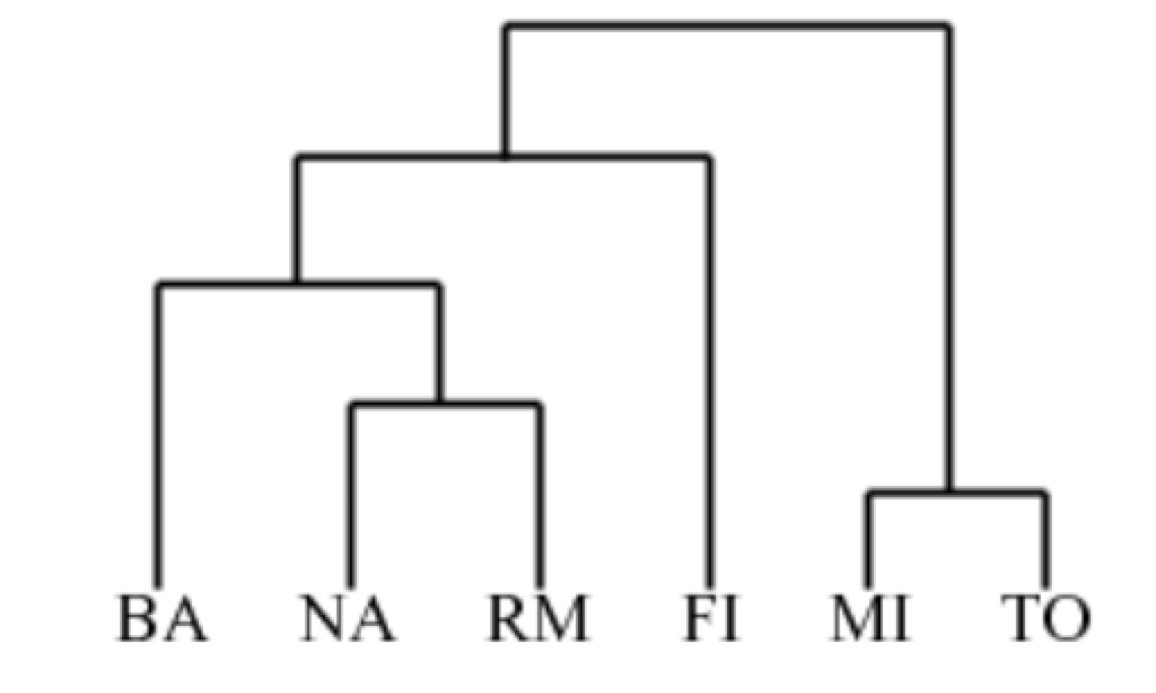
\includegraphics[scale=.3]{dend1.png}
\end{center}
Using this dendrogram to create 3 clusters, what would the clusters be?
}}{
\MCOption[2.5in]{\{BA,NA\},\{RM,FI\},\{MI,TO\}} 
\MCOption[2.5in]{\{NA,RM\},\{BA,FI\},\{MI,TO\}} \\
\MCOption[2.5in]{\{BA,NA,RM,FI\},\{MI\},\{TO\}} 
\MCOption[2.5in]{\{BA,NA,RM\},\{FI\},\{MI, TO\}} \\
}\\


%
%\item \QuizQ{ \TextInBoxOne{5.4in}{
%One of the primary assumptions of the standard linear regression is the Normality of the corresponding errors.  Based on the the visual inspection of the standard  residual plot, a practitioner suspects that the assumption on the  independence of the model errors may not be satisfied for the dataset.  Therefore,  he/she conducts the standard Durbin-Watson Test of the corresponding residuals and obtained a p-value of $0.37$.  What can be concluded from the above information:
%}}{
%Ans:\\
%\MCOption[5in]{The  model residuals may not be correlated.  } \\
% \MCOption[5in]{There is a Strong Statistical Evidence that the residuals are correlated. }
% \MCOption[5in]{There is a some Statistical Evidence that the residuals are correlated. }
%}\\

% 
%
%\item \QuizQ{ \TextInBoxOne{5.4in}{
%In the context of Standard Linear Regression to model a continuous response variable, how do we check if there is 'Influential' point in the dataset. 
%}}{Ans: \\
% \MCOption[5in]{It is a Influential point if the corresponding Cook's Distance is more than 0.5. }
%\MCOption[5in]{It is a Influential point if the corresponding Cook's Distance is less than 0.5. }
%\MCOption[5in]{It is a Influential point if the corresponding Cook's Distance is less than 0.05. }
%}\\


%\item \QuizQ{ \TextInBoxOne{5.4in}{
%Question whether to apply logistic regression or Linear Regression
%}}{
%
%}\\


%\item \QuizQ{ \TextInBoxOne{5.4in}{
%{\bf Statement: } AIC BASED model selection
%}}{
%Ans:\MCOption{TURE} \MCOption{FALSE}
%}\\



%
%\item \QuizQ{ \TextInBoxOne{5.4in}{
%If we consider a 3 degree regression splines with 7 knot points, then how many regression coefficient parameters are there in the model? (i.e.  what is the dimension of the model?)
%}}{
%Ans:\MCOption[1in]{20}\MCOption[1in]{11}  \MCOption[1in]{9}\MCOption[1in]{10}
%}\\

%
%\item \QuizQ{ \TextInBoxOne{5.4in}{
%Calculate Complete Linkage
%}}{
%Ans:\MCOption[1in]{24}\MCOption[1in]{16}  \MCOption[1in]{30}\MCOption[1in]{76}
%}\\


%
%
%\item \QuizQ{ \TextInBoxOne{5.4in}{
%Two different set of knots
%}}{
%
%}\\

%\item \QuizQ{ \TextInBoxOne{5.4in}{ Let $\pi\in (0,1)$ such that  $\text{Logit}(\pi)=1.12$.  What is the most appropriate value of $\pi$ from the list below. 
%}}{
%\MCOption[1in]{$0.543$}  \MCOption[1in]{$0.97$} \MCOption[1in]{$0.754$}\MCOption[1in]{$3.065$}
%}\\
%
%\item \QuizQ{ \TextInBoxOne{5.4in}{ Let $x$ be a real number such that  $\text{Expit}(x)=0.65$.  What is the most appropriate value of $x$ from the list below. 
%}}{
%\MCOption[1in]{$0.268$}  \MCOption[1in]{$-0.187$} \MCOption[1in]{$1.916$}\MCOption[1in]{$3.065$}
%}\\
%
%
%\item \QuizQ{ \TextInBoxOne{5.4in}{ Let $\pi\in (0,1)$ such that  $\text{Logit}(\pi)=2.5$.  What is the most appropriate value of $\text{Odds}(\pi)$ from the list below. 
%}}{
%\MCOption[1in]{$0.924$}  \MCOption[1in]{$12.18$} \MCOption[1in]{$0.397$}\MCOption[1in]{$9.11$}
%}\\

\item \QuizQ{ \TextInBoxOne{5.4in}{ In order to model a multi-category response variable, a classification tree is utilized.  Let the response variable can take only 4 categories.  During the modeling, a specific terminal node of the tree has the corresponding proportion/ probabilities to be $\hat{\pi}=(0.1, 0.8, 0.04, 0.06)^T$ to the different response categories for the points assigned to it.  Calculate the 
Gini's Index for the obtained probability vector.
}}{
Ans: \vspace{.5in}
}\\

\item \QuizQ{ \TextInBoxOne{5.4in}{ In order to model a multi-category response variable, a classification tree is utilized.  Let the response variable can take only 4 categories.  During the modeling, a specific terminal node of the tree has the corresponding proportion/ probabilities to be $\hat{\pi}=(0.08, 0.81, 0.05, 0.06)^T$ to the different response categories for the points assigned to it.  Calculate the 
Cross-Entropy Index for the obtained probability vector.
}}{
Ans: \vspace{.5in}
}\\


\item \QuizQ{ \TextInBoxOne{5.4in}{ In order to model a multi-category response variable, a classification tree is utilized.  Let the response variable can take only 4 categories.  During the modeling, a specific terminal node of the tree has the corresponding proportion/ probabilities to be $\hat{\pi}=(0.15, 0.1 0.65, 0.1)^T$ to the different response categories for the points assigned to it.  Calculate the 
mis-classification rate for the obtained probability vector.
}}{
Ans: \vspace{.5in}
}\\
%\item \QuizQ{ \TextInBoxOne{5.4in}{
%In a game of rolling a fair dice twice. A player wins if both throws result in  sixes. What is the odds of winning the game?
%}}{
%Ans:  \MCOption[1in]{$\frac{1}{36}$}\MCOption[1in]{$\frac{1}{6}$}  \MCOption[1in]{$\frac{1}{35}$}\MCOption[1in]{$\frac{35}{36}$}
%}\\
%
%
%
%
%\item \QuizQ{ \TextInBoxOne{5.4in}{
%Imagine we have a sample of 150 points, 70 from ‘Class 0’ ( For example: healthy) and the others from ‘Class 1 ( For Example: Not Healthy). Let us assume that a classification technique (Medical Testing) can correctly identify 65 out of the 70 belongs to the ‘Class 0’ (positive for all Diseased) while it can correctly detect 77 of objects that belongs to the ’Class1’(Not Healthy). Calculate the {\bf Sensitivity}  for the corresponding Classification Technique. 
%}}{
%\MCOption[1in]{$96.25\%$}\MCOption[1in]{$91.31\%$}  \MCOption[1in]{$92.92\%$}\MCOption[1in]{$93.90\%$}
%}\\
%
%
%
%\item \QuizQ{ \TextInBoxOne{5.4in}{
%Imagine we have a sample of 150 points, 70 from ‘Class 0’ ( For example: healthy) and the others from ‘Class 1 ( For Example: Not Healthy). Let us assume that a classification technique (Medical Testing) can correctly identify 65 out of the 70 belongs to the ‘Class 0’ (positive for all Diseased) while it can correctly detect 77 of objects that belongs to the ’Class1’(Not Healthy). Calculate the {\bf Specificity}  for the corresponding Classification Technique. 
%}}{
%\MCOption[1in]{$96.25\%$}\MCOption[1in]{$95.59\%$}  \MCOption[1in]{$92.85\%$}\MCOption[1in]{$93.90\%$}
%}\\
%
%\item \QuizQ{ \TextInBoxOne{5.4in}{
%Imagine we have a sample of 150 points, 70 from ‘Class 0’ ( For example: healthy) and the others from ‘Class 1 ( For Example: Not Healthy). Let us assume that a classification technique (Medical Testing) can correctly identify 65 out of the 70 belongs to the ‘Class 0’ (positive for all Diseased) while it can correctly detect 77 of objects that belongs to the ’Class1’(Not Healthy). Calculate the {\bf Yuden Index } for the corresponding Classification table. 
%}}{
%\MCOption[1in]{$0.891$}\MCOption[1in]{$0.938$}  \MCOption[1in]{$0.929$}\MCOption[1in]{$1.86$}
%}\\
%
%
%\item \QuizQ{ \TextInBoxOne{5.4in}{
%Imagine we have a sample of 150 points, 70 from ‘Class 0’ ( For example: healthy) and the others from ‘Class 1 ( For Example: Not Healthy). Let us assume that a classification technique (Medical Testing) can correctly identify 65 out of the 70 belongs to the ‘Class 0’ (positive for all Diseased) while it can correctly detect 77 of objects that belongs to the ’Class1’(Not Healthy). Calculate the Yuden Index for the corresponding Classification table. 
%}}{
%\MCOption[1in]{$0.891$}\MCOption[1in]{$0.938$}  \MCOption[1in]{$0.929$}\MCOption[1in]{$1.86$}
%}\\
%
%\item \QuizQ{ \TextInBoxOne{5.4in}{
%Consider analyzing a data-set that has a binary categorical response while all the covariates are numerical and continuous in nature.  We know that a logistic regression and also a quadratic discriminant analysis is applied for  modeling the response variable.  To compare the performance of both the method a ROC curve is constructed and the corresponding Area Under the ROC Curve (AUC) is calculated based on their performance in a Testing set. The AUC for the logistic regression is 0.91 while the AUC for the QDA is 0.85.  Identify whether the following statement is TRUE or FALSE. 
%{\bf Statement: } The Logistic regression is performing bettern then that of the QDA for this data set that is evaluated based on the testing set. 
%}}{
%\MCOption[1in]{TRUE}\MCOption[1in]{FALSE} 
%}\\
%
%
%
%





\end{enumerate}


\newpage
 
 
 
 

\DefBoxOne{}{
\begin{center}\color{black}
Part II:  Descriptive Problems. 
\end{center}
}
%\DefBoxOne{Notations}{
%$$ \Onebf_k=\left[ \begin{array}{c}1\\1\\\vdots \\1\end{array}\right]_{k\times 1} \text{ , }  J_{k}=\left[ \begin{array}{cccc}1&1 & \cdots & 1\\1& 1& \cdots&  1\\\vdots & \vdots & \ddots  &\vdots \\1& 1 &\cdots & 1\end{array}\right]_{k\times k} \text{ and } I_{k}=\left[ \begin{array}{cccc}1&0 & \cdots & 0\\0& 1& \cdots&  0\\\vdots & \vdots & \ddots  &\vdots \\0& 0 &\cdots & 1\end{array}\right]_{k\times k} \text{ for } k\in \Z_{+}.   $$
%
%}
\begin{enumerate}
\item {\Large Must Review: Review All the Quiz Problems. Also Review all the problems in the problem set that we have circulated before the midterm.}
\item \QuizQ{ \TextInBoxOne{5.4in}{
Consider a clustering problem of bi-variate data with the following distance matrix: \\
\begin{center}
\begin{tabular}{|l|l|l|l|l|l|}
\hline
 & A   & B   & C   & D   & E   \\ \hline
A & 0   & 6.5 & 2.4 & 4.2 & 5.9 \\ \hline
B & 6.5 & 0   & 4.7 & 4.5 & 2.8 \\ \hline
C & 2.4 & 4.7 & 0   & 2.4 & 4.1 \\ \hline
D & 4.2 & 4.5 & 2.4 & 0   & 1.7 \\ \hline
E & 5.9 & 2.8 & 4.1 & 1.7 & 0   \\ \hline
\end{tabular}
\end{center}
Point names are denoted by the Letters $A,B,C,D,E$.
\begin{enumerate}
\item Construct a Dendogram for hierarchical agglomerative clustering  using the {\bf complete-linkage} procedure.
\item Identify the cluatering assignment of the points if one decides to split the data into two clusters. 
\end{enumerate}
}}{

}\\

Ans: 






%\newpage 
%\item \QuizQ{ \TextInBoxOne{5.4in}{
%Consider a clustering problem of bi-variate data with the following distance matrix: \\
%\begin{center}
%\begin{tabular}{|l|l|l|l|l|l|}
%\hline
%  & A   & B   & C   & D   & E   \\ \hline
%A & 0   & 4.9 & 5.6 & 1.3 & 4.2 \\ \hline
%B & 4.9 & 0   & 5.9 & 3.6 & 4.5 \\ \hline
%C & 5.6 & 5.9 & 0   & 5.3 & 2.6 \\ \hline
%D & 1.3 & 3.6 & 5.3 & 0   & 3.9 \\ \hline
%E & 4.2 & 4.5 & 2.6 & 3.9 & 0   \\ \hline
%\end{tabular}
%\end{center}
%Point names are denoted by the Letters $A,B,C,D,E$.
%\begin{enumerate}
%\item Construct a Dendogram for hierarchical agglomerative clustering  using the {\bf single-linkage} procedure.
%\item Identify the clustering assignment of the points if one decides to split the data into two clusters. 
%\end{enumerate}
%}}{
%
%}\\

\newpage 
\item \QuizQ{ \TextInBoxOne{5.4in}{
Consider a clustering problem of bi-variate data
$$A=\ColVec{4,3},
B=\ColVec{2,2},
C=\ColVec{2,6},
D=\ColVec{5,0},
E=\ColVec{0,3},
F=\ColVec{4,0}, $$
where the points are labeled as A, B, C, D, E, F. The Euclidean distance between the points are provided in the distance matrix below:
\begin{center}
\begin{tabular}{|l|l|l|l|l|l|l|}
\hline
  & A    & B    & C    & D    & E    & F    \\ \hline
A & 0    & 2.24 & 3.61 & 3.16 & 4    & 3    \\ \hline
B & 2.24 & 0    & 4    & 3.61 & 2.24 & 2.83 \\ \hline
C & 3.61 & 4    & 0    & 6.71 & 3.61 & 6.32 \\ \hline
D & 3.16 & 3.61 & 6.71 & 0    & 5.83 & 1    \\ \hline
E & 4    & 2.24 & 3.61 & 5.83 & 0    & 5    \\ \hline
F & 3    & 2.83 & 6.32 & 1    & 5    & 0    \\ \hline
\end{tabular}
\end{center}
\vspace{.2in}
 During an iteration of the K-means algorithm with 2 clusters, the points $\{A,D,F\}$ are assigned to Cluster1 and the rest of the points to the Cluster2. 
\begin{enumerate}
\item  Identify the resulting cluster centers for both the groups at the beginning   of the next iteration.
\item Compute the Withing Group Sum of Squares for  clusters provided in part(a).  Note that,  you may take help from the provided distance matrix. 
\end{enumerate}
}}{

}\\



%\item \QuizQ{ \TextInBoxOne{5.4in}{
%Provide Spectral Decomposition and Ask Questions on Principal components
%\begin{enumerate}
%\item Question 1
%\item Question2
%\end{enumerate}
%}}{
%
%}\\
%








\item \QuizQ{ \TextInBoxOne{5.4in}{
Consider a dataset that includes data on 150 diamonds sold at an auction.  We applied a regression-tree  model to  build a  model to  predict the price of a diamond  based on the 'weight',  `clarity', and `color' of a diamond.  
The variables that are present in the data are the following: \\
{\bf "value":} The price at which the diamond is sold.  (in $10^5$ USD)\\
{\bf "weight"}: Weight of the diamond.  (grams)\\
{\bf  "clarity"}: Clarity measure of the diamond.(A score between 0 to 2)\\
   {\bf "color" }: Color of the diamond. (A score between 1 to 10)\\
       

The following is the diagram of the obtained tree that we denote here by $\text{T}^{*}$ when modeling the continuous variable 'value':\\
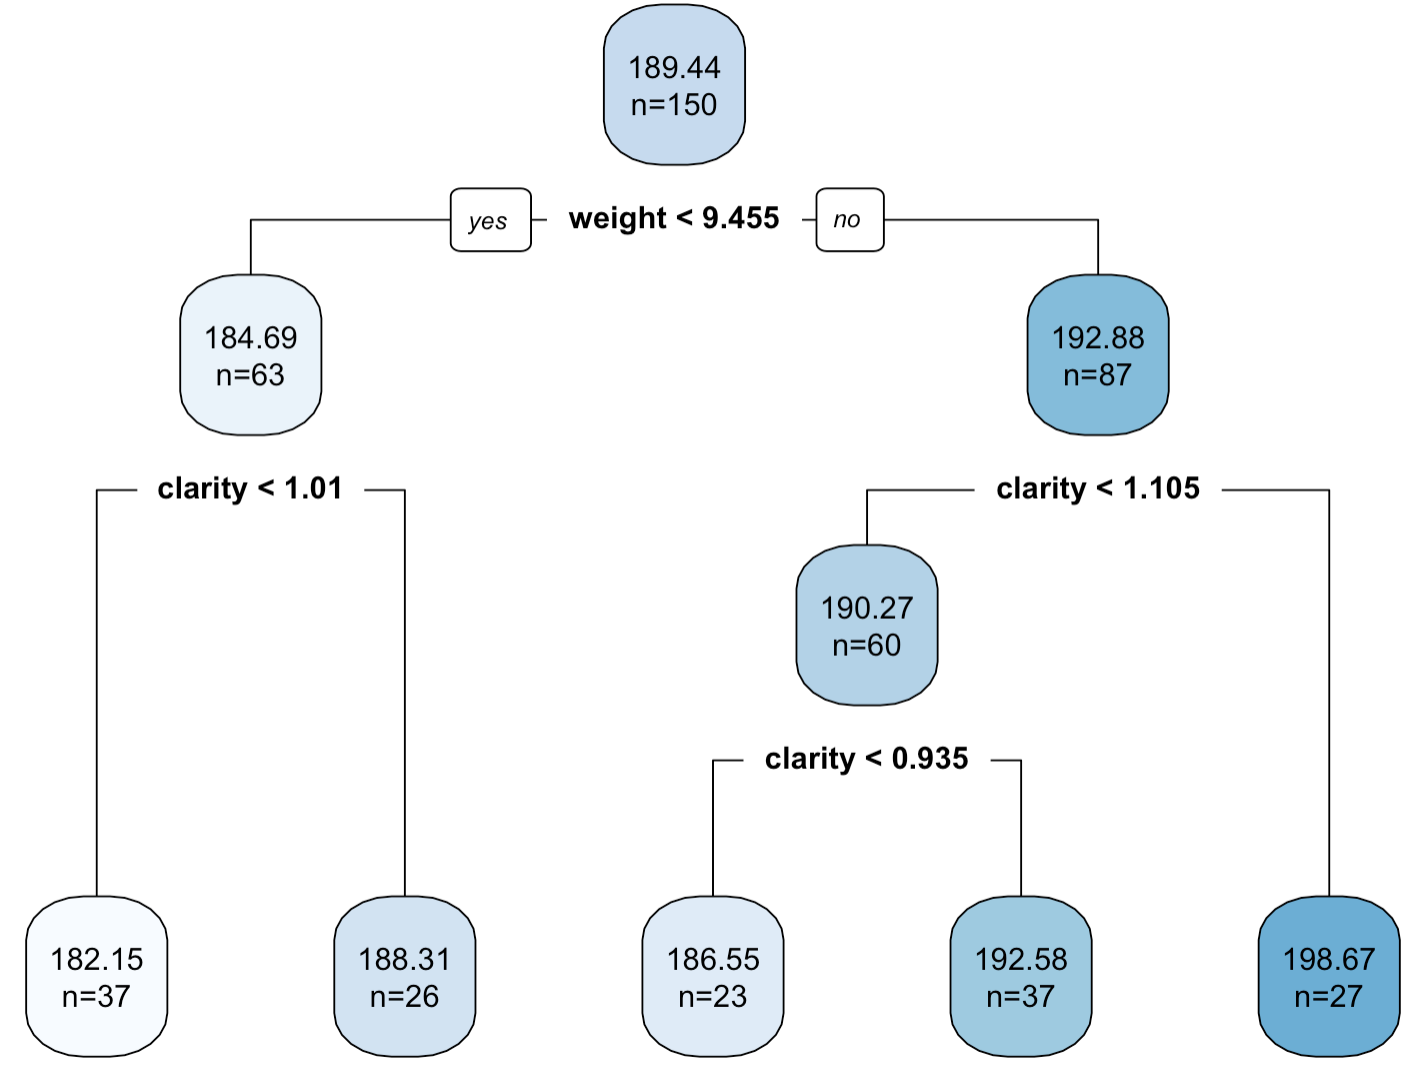
\includegraphics[scale=.55]{TreeDiamond.png}
The numbers provided at the terminal node,  denote the the corresponding predicted response ans the number of observations are allocated to the specific terminal node.  Answer the following questions based on the estimated tree given in this problem. 
\begin{enumerate}
\item Let $ \alpha(\text{T})$ denote the usual complexity measure obtained by the number of the terminal node of the tree or the number of decision regions that it corresponds.  What is the value of $\alpha(\text{T}^{*})$?
\item Write down/Describe the  different decision regions that the tree corresponds to. 

\item What would be predicted response of a point that has the following values for the corresponding covariates\\
{\small
 \begin{tabular}{|l|l|l|l|l|l|l|l|l|l|l|l|l|}
\hline
crim & zn   & indus & chas & nox  & rm   & age  & dis & rad & tax & ptratio & lstat & medv \\ \hline
0.17 & 12.5 & 7.87  & 0    & 0.53 & 6.01 & 85.9 & 6.5 & 5   & 311 & 15.2    & 17.1  &  ?    \\ \hline
\end{tabular}
}
\end{enumerate}
}}{

}\\





%
%
%\item \QuizQ{ \TextInBoxOne{5.4in}{
%Provide R output of clustering and Ask Questions
%\begin{enumerate}
%\item 
%\item 
%
%\item
%\end{enumerate}
%}}{
%
%}\\
%
%
%
%
%
%\item \QuizQ{ \TextInBoxOne{5.4in}{
%Tree Complexity question  and pruning tree
%\begin{enumerate}
%\item 
%\item 
%
%\item
%\end{enumerate}
%}}{
%
%}\\
%
%
%
%
%\item \QuizQ{ \TextInBoxOne{5.4in}{
%
%\begin{enumerate}
%\item 
%\item 
%
%\item
%\end{enumerate}
%}}{
%
%}\\
%
%
%
%
%\item \QuizQ{ \TextInBoxOne{5.4in}{
%
%\begin{enumerate}
%\item 
%\item 
%
%\item
%\end{enumerate}
%}}{
%
%}\\

%
%
%\item \QuizQ{ \TextInBoxOne{5.4in}{
%Question random forest
%\begin{enumerate}
%\item 
%\item 
%
%\item
%\end{enumerate}
%}}{
%
%}\\



\item \QuizQ{ \TextInBoxOne{5.4in}{
Consider a small data set of 6 observations: \\
\begin{tabular}{|l|l|l|l|l|l|}
\hline
DataId & Sepal.Length & Sepal.Width & Petal.Length & Petal.Width & Species    \\ \hline
1      & 6.5          & 3           & 5.2          & 2           & virginica  \\ \hline
2      & 5.1          & 3.5         & 1.4          & 0.2         & setosa     \\ \hline
3      & 7            & 3.2         & 4.7          & 1.4         & versicolor \\ \hline
4      & 4.9          & 3           & 1.4          & 0.2         & setosa     \\ \hline
5      & 5.8          & 2.7         & 5.1          & 1.9         & virginica  \\ \hline
6      & 4.6          & 3.4         & 1.4          & 0.3         & setosa     \\ \hline
\end{tabular}
The objective of this problem is to obtain a bootstrap sample of the above data.  As we have only 6 observations here, we may assume that a random data row can be selected by rolling a dice.  In particular,  we can select the specific DataId that matches with the number that appears as a result of the throw of the dice.  The following is the results of 10 independent throws of a dice: 
$$\{ 5,  3,  4,  1 , 2,  4,  5,  1, 6 , 1\}$$


\begin{enumerate}
\item Obtain a Bootstrap sample of the above data. Clearly indicate which DataId's are you selecting.  
\end{enumerate}
}}{

}\\




\item \QuizQ{ \TextInBoxOne{5.4in}{
Let $\hat{\Sigma}$ be an estimated variance covariance matrix from a data set.  As the variance covariance matrix is non negative definite matrix, a spectral decomposition of the matrix is possible to be done.  Based on a computation procedure to applied to  $\hat{\Sigma}$, the following spectral decomposition is obtained:
$$\hat{\Sigma}:=\Gamma \Lambda \Gamma^T, \text{ where }$$

$$\Gamma=\RowVec{ \Col{0.78,0.24,0.37,0.06,-0.32,0.3,-0.06,-0.01} , \Col{-0.06,-0.33,0.66,0.22,0.21,-0.15,0.37,-0.46} , \Col{-0.04,0.78,-0.14,0.35,0.19,-0.21,0.05,-0.4} , \Col{-0.38,0.03,0.04,0.57,-0.61,0.21,0.25,0.21} , \Col{-0.26,0.27,0.45,-0.42,-0.42,-0.52,-0.19,0.1} , \Col{-0.13,0.25,0.41,0.17,0.52,0.14,-0.08,0.65} , \Col{-0.32,-0.03,0.18,0.05,0,0.46,-0.72,-0.37} , \Col{0.25,-0.29,-0.06,0.54,-0.01,-0.55,-0.49,0.13} }$$
$$\Lambda=\RowVec{ \Col{20,0,0,0,0,0,0,0} , \Col{0,15,0,0,0,0,0,0} , \Col{0,0,1.1,0,0,0,0,0} , \Col{0,0,0,0.9,0,0,0,0} , \Col{0,0,0,0,0.8,0,0,0} , \Col{0,0,0,0,0,0.5,0,0} , \Col{0,0,0,0,0,0,0.02,0} , \Col{0,0,0,0,0,0,0,0.001} }.$$
Note that $\Gamma$ is an Orthogonal-Matrix i.e. $\Gamma^T\Gamma=\Gamma\Gamma^T=\text{I}_{_{8\times 8}}$ while,  $\Lambda$ is a diagonal matrix with non-negative diagonal elements.  Also, note that the columns of the matrix $\Gamma$ comprises of the eigen-vectors of the matrix $\hat{\Sigma}$ while the diagonal elements of the matrix $\Lambda$ refers to the corresponding eigen-values of $\hat{\Sigma}$. Answer the following questions based on the results provided above.

\begin{enumerate}
\item   Derive the equation for the first three principal components of the observed data.  i.e.  What is the equation for the first three principal components, $\text{PC}_1$, $\text{PC}_2$, and $\text{PC}_3$, of the observed data? 
\item What is the loading of $\text{PC}_{1}$ on the different variables?
\item Derive the variance of $\text{PC}_{1}$.
\item Derive the co-variance between  $\text{PC}_{1}$ and $\text{PC}_{2}$.

\item Draw a scree plot of the importance factors for the principal components.  Based on the scree-plot,  identify the optimum number of components (say $m$) that would be adequate to capture the variability present in the observed data.  

\item  What is the  percentage of total variability that is captured by the first $m$ principal components of the data.  
\item If a specific observed data point is 
$X_ 1 = 2.44,X_ 2 = 4.82,X_ 3 = 2.43,X_ 4 = -0.2,X_ 5 = -0.29,X_ 6 = -3.32,X_ 7 = 1.77,X_ 8 = -7.65$
What is the score of the plot along the first two principal components?
\end{enumerate}
}}{

}\\





\item \QuizQ{ \TextInBoxOne{5.4in}{
Let $\hat{\Sigma}$ be an estimated variance covariance matrix from a data set.  As the variance covariance matrix is non negative definite matrix, a spectral decomposition of the matrix is possible to be done.  Based on a computation procedure to applied to  $\hat{\Sigma}$, the following spectral decomposition is obtained:
$$\hat{\Sigma}:=\Gamma \Lambda \Gamma^T, \text{ where }$$

$$\Gamma=\RowVec{ \Col{0.15,0.58,-0.06,-0.05,0.8} , \Col{0.93,0.03,0.28,0.14,-0.17} , \Col{0.11,0.22,-0.8,0.51,-0.22} , \Col{0.28,-0.21,-0.52,-0.78,0.01} , \Col{0.11,-0.76,-0.13,0.33,0.53} }$$
$$\Lambda=\RowVec{ \Col{12,0,0,0,0} , \Col{0,6,0,0,0} , \Col{0,0,1,0,0} , \Col{0,0,0,0.9,0} , \Col{0,0,0,0,0.1} }.$$
Note that $\Gamma$ is an Orthogonal-Matrix i.e. $\Gamma^T\Gamma=\Gamma\Gamma^T=\text{I}_{_{5\times 5}}$ while,  $\Lambda$ is a diagonal matrix with non-negative diagonal elements.  Also, note that the columns of the matrix $\Gamma$ comprises of the eigen-vectors of the matrix $\hat{\Sigma}$ while the diagonal elements of the matrix $\Lambda$ refers to the corresponding eigen-values of $\hat{\Sigma}$. Answer the following questions based on the results provided above.

\begin{enumerate}
\item   Derive the equation for the first three principal components of the observed data.  i.e.  What is the equation for the first three principal components, $\text{PC}_1$, $\text{PC}_2$, and $\text{PC}_3$, of the observed data? 
\item What is the loading of $\text{PC}_{1}$ on the different variables?
\item Derive the variance of $\text{PC}_{1}$.
\item Derive the co-variance between  $\text{PC}_{1}$ and $\text{PC}_{2}$.

\item Draw a scree plot of the importance factors for the principal components.  Based on the scree-plot,  identify the optimum number of components (say $m$) that would be adequate to capture the variability present in the observed data.  

\item  What is the  percentage of total variability that is captured by the first $m$ principal components of the data.  
\item If a specific observed data point is 
$X_ 1 = 2.44,X_ 2 = 4.82,X_ 3 = 2.43,X_ 4 = -0.2,X_ 5 = -0.29$
What is the score of the plot along the first two principal components?
\end{enumerate}
}}{

}\\




\item \QuizQ{ \TextInBoxOne{5.4in}{
Consider the following diagram of a Perceptron:\\
\begin{center}
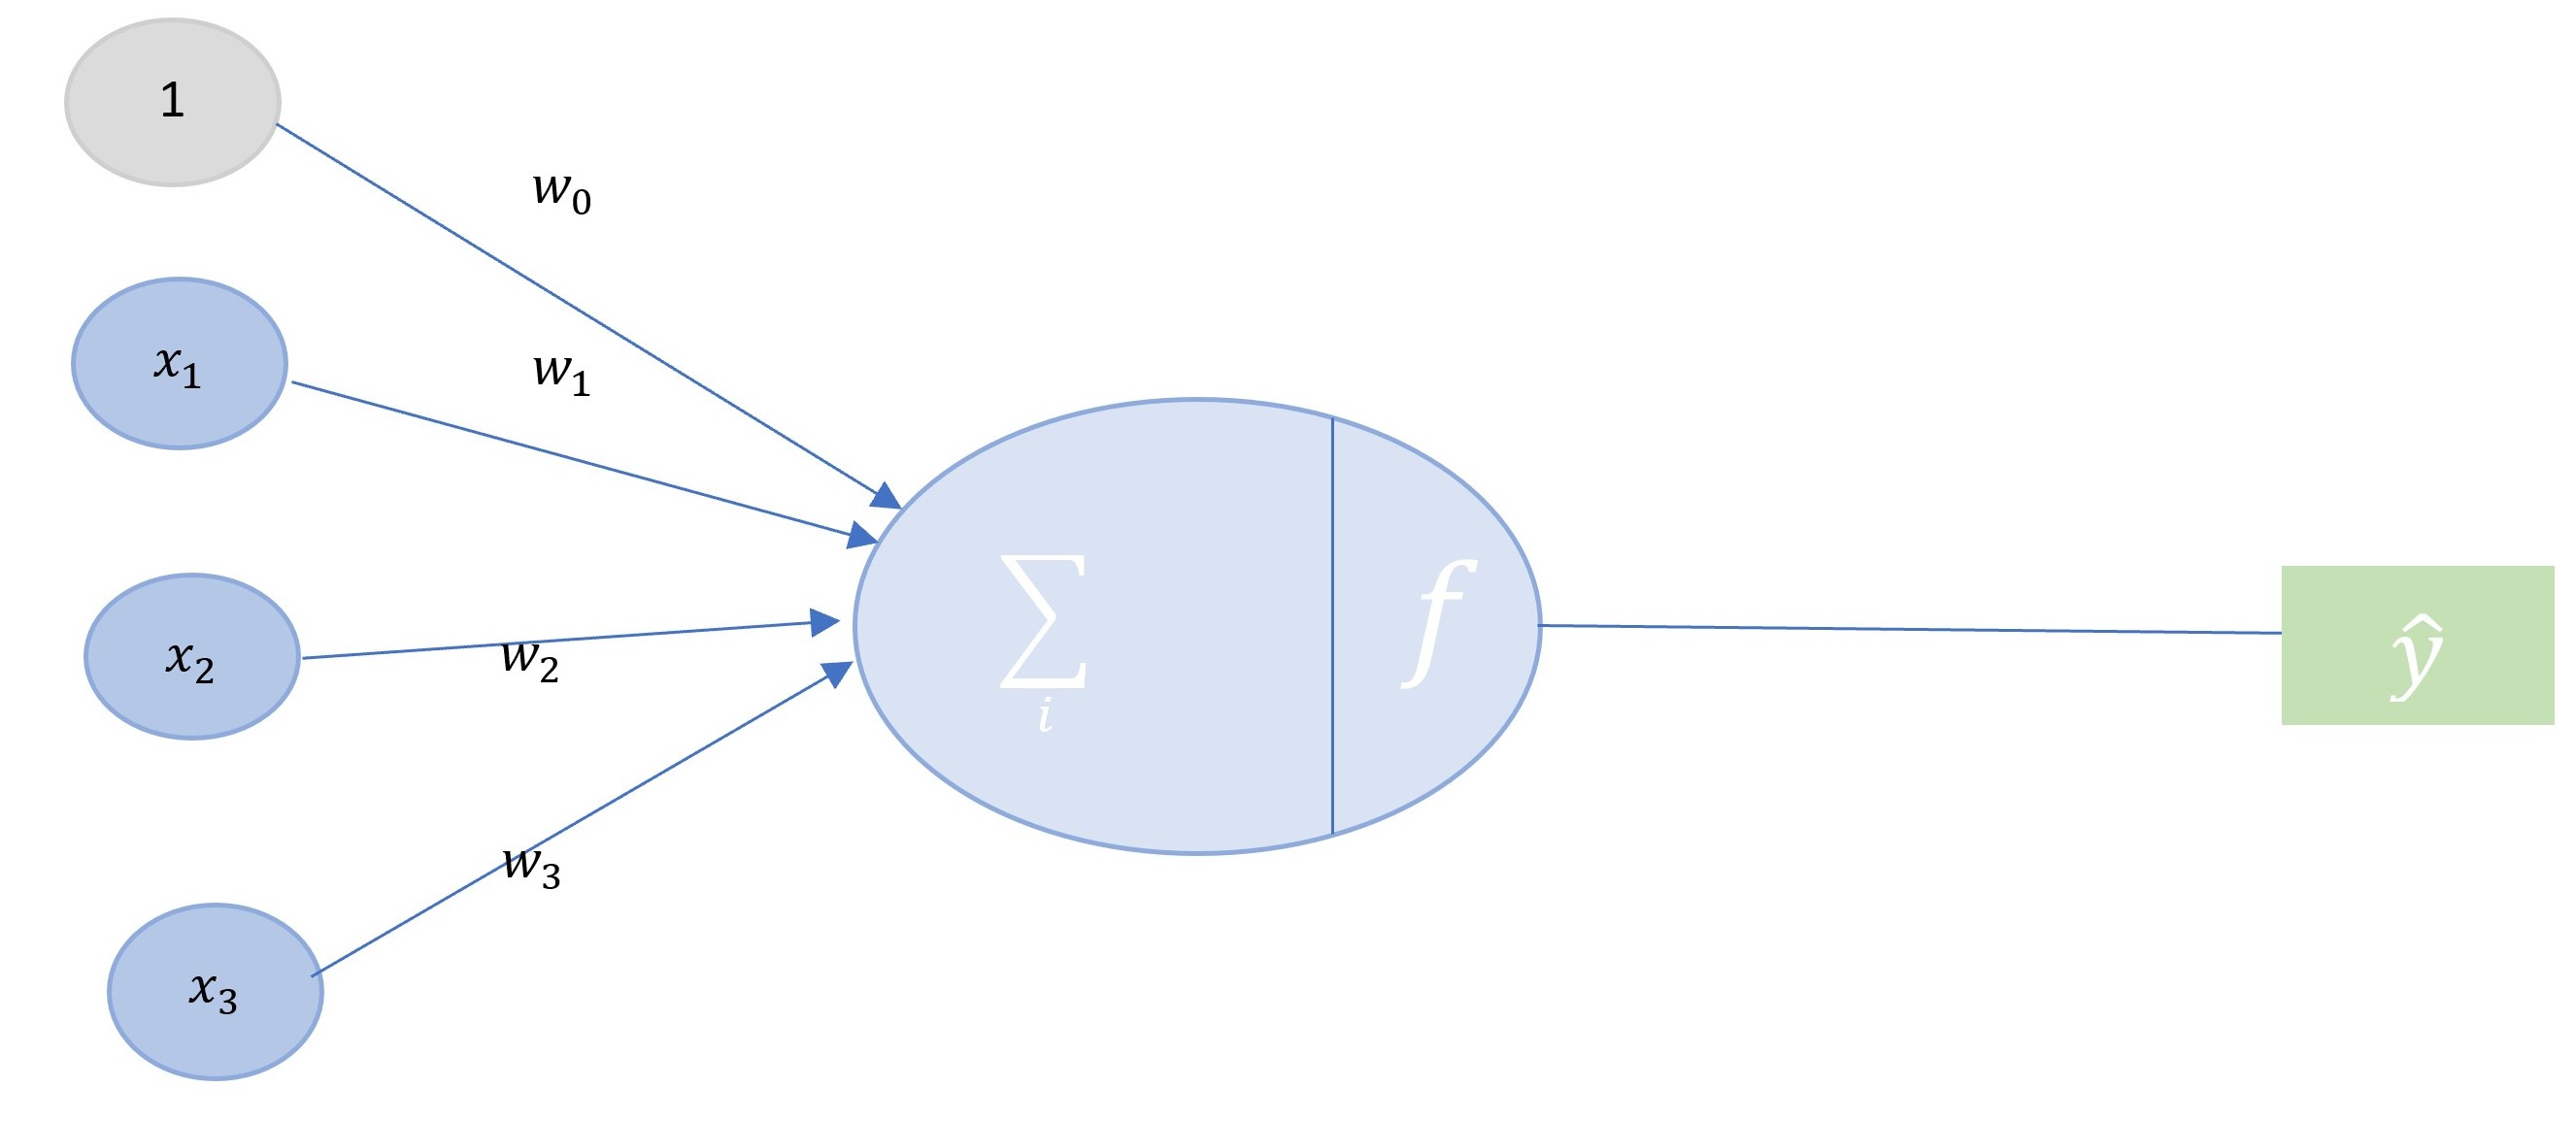
\includegraphics[scale=.38]{Perceptron_img.jpg}
\end{center}
Let the weights are given to be $\w_0=5$, $\w_1=2$, $\w_2=-3$, $\w_3=1$.  The observed covariates/imputs are given as
$x_1=4, x_2=1, X_3=-1$.  
\begin{enumerate}
\item Write down the mathemetical formulation of the above Perceptron.  Keep the nonlinear function to be the generic $f$ in your expression.
\item If we consider the nonlinear function $f$ to be the Sigmoid function, then what would be the output from the above Perceptron?
\item If we consider the nonlinear function $f$ to be the ReLU function, then what would be the output from the above Perceptron?
\end{enumerate}
}}{

}\\


\vspace{1.5in}
\item \QuizQ{ \TextInBoxOne{5.4in}{
Consider the dendrogram: \\
\begin{center}
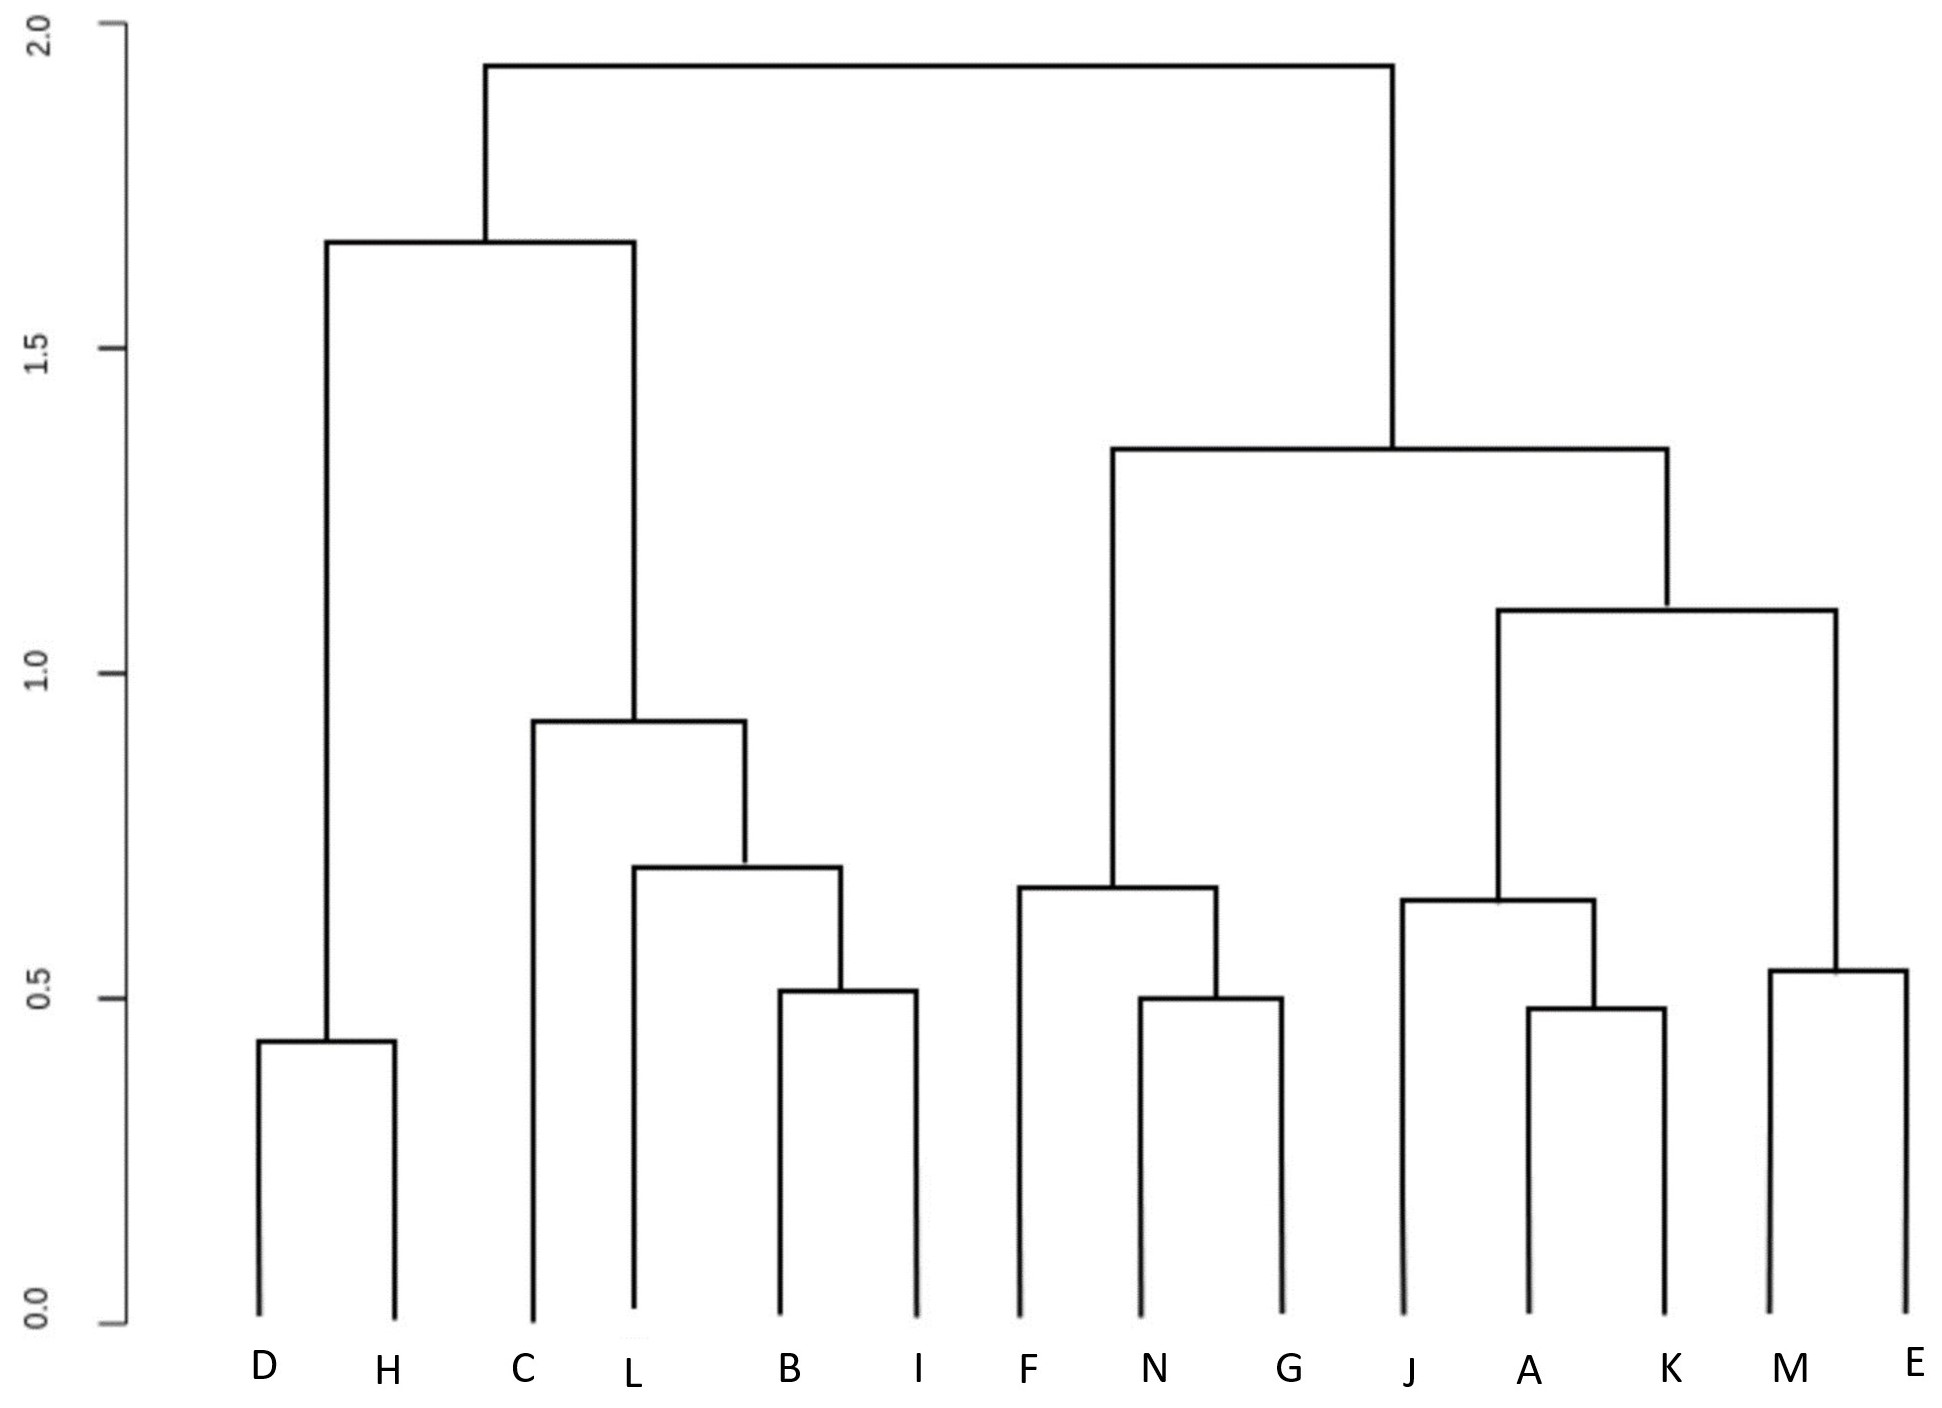
\includegraphics[scale=.39]{dendo_2.jpg}
\end{center}
Using this dendrogram to create 4 clusters, what would the clusters be?
}}{
\begin{enumerate}
\item Identify the clusters if it is given that there is only three clusters. 
\item Identity the two points which are closest to each other. 
\end{enumerate}
}\\


\end{enumerate}






\end{document}